\documentclass[11pt,a4paper,reqno]{amsart}

\usepackage{amsmath}
\usepackage{amssymb}
\usepackage{amsthm}
\usepackage[shortlabels]{enumitem}
\usepackage[british]{babel}
\usepackage{microtype}
\usepackage{needspace}
\usepackage{tikz}
\usepackage{booktabs}
\usepackage{xcolor}
\usepackage{hyperref}

\setlength{\textwidth}{\paperwidth}
\addtolength{\textwidth}{-2.5in}
\calclayout
\setlist[enumerate]{leftmargin=2.2em,itemsep=2pt,topsep=4pt}
\hypersetup{
 colorlinks=true,
 linkcolor=blue!45!black,
 citecolor=blue!45!black,
 urlcolor=blue!45!black,
 pdftitle={Global weak Euler flows with finite signed initial vorticity},
 pdfauthor={},
 pdfsubject={Weak Euler solutions, signed measure vorticity, and stress repair preserving endpoint velocities},
 pdfkeywords={Euler equations, vortex sheets, convex integration, signed vorticity, Biot-Savart},
}

\theoremstyle{plain}
\newtheorem{theorem}{Theorem}[section]
\newtheorem{lemma}[theorem]{Lemma}
\newtheorem{proposition}[theorem]{Proposition}
\newtheorem{corollary}[theorem]{Corollary}
\newtheorem{conjecture}[theorem]{Conjecture}
\theoremstyle{definition}
\newtheorem{definition}[theorem]{Definition}
\theoremstyle{remark}
\newtheorem{remark}[theorem]{Remark}
\numberwithin{equation}{section}

\newcommand{\R}{\mathbb R}
\newcommand{\M}{\mathcal M}
\newcommand{\X}{\mathcal X}
\newcommand{\PP}{\mathbb P}
\newcommand{\curl}{\operatorname{curl}}
\newcommand{\Div}{\operatorname{div}}
\newcommand{\supp}{\operatorname{supp}}
\newcommand{\norm}[2]{\left\|#1\right\|_{#2}}
\newcommand{\dd}{\,dx}
\newcommand{\ee}{\mathrm e}
\newcommand{\ind}{\mathbf 1}
\newcommand{\doi}[1]{\href{https://doi.org/#1}{\nolinkurl{#1}}}

% The author information is intentionally left blank.
% Add this paper's author, address, and email here when ready.
% \author{Author name}
% \address{Department and institution}
% \email{author@example.org}
\title[Weak Euler flows with signed initial vorticity]{Global weak Euler flows with\\
finite signed initial vorticity}
\date{}
\keywords{Euler equations, vortex sheets, convex integration, signed vorticity, Biot--Savart}

% Permit a long display to break between lines.
\allowdisplaybreaks[1]

\begin{document}

\begin{abstract}
We construct infinitely many global weak solutions of the
two-dimensional Euler equations on the plane for every finite signed
initial vorticity $\mu_0$ in the inhomogeneous space $H^{-1}$. The
velocity approaches its Biot--Savart initial value $u_0=K*\mu_0$ in
the sense that $\|u(t)-u_0\|_{L^2}\to0$ as $t\downarrow0$, although
$u_0$ itself need not belong to $L^2$. The vorticity is integrable at
every positive time, continuous into $H^{-1}$, and weakly-* continuous
as a finite measure. For an $L^1$ initial density, it is strongly
continuous in $L^1$ up to the initial time. We first construct an
approximate Euler flow whose stress tends to zero at the initial
time. We then remove this stress using moving dipoles, with
corrections that are summable in velocity $L^2$ and vorticity $L^1$.
The corrections leave the velocity unchanged at the endpoints of each
time interval. Nonzero circulation is allowed. No energy inequality,
sign preservation, or Lagrangian transport property is imposed.
\end{abstract}

\maketitle

\section{Introduction}\label{sec:intro}

The two-dimensional Euler equations describe the motion of an ideal
incompressible fluid:
\begin{equation}\label{eq:euler-intro}
 \partial_tu+\Div(u\otimes u)+\nabla p=0,
 \qquad \Div u=0.
\end{equation}
Here $u$ is the velocity and $p$ is the pressure. For a smooth solution,
the scalar vorticity $\omega=\partial_1u_2-\partial_2u_1$ satisfies
\[
 \partial_t\omega+u\cdot\nabla\omega=0.
\]
The absence of vortex stretching is the basic reason that the planar
problem has a global classical theory. It does not, however, settle the
existence problem for singular vorticity. A vortex sheet carries
vorticity on a curve, rather than on a set of positive area. More
generally, the initial vorticity may be a finite signed measure. The
question is then whether such data generate a velocity solving the
nonlinear Euler equation, and in what class that velocity should be
sought.

For compactly supported measures, membership in $H^{-1}(\R^2)$ is the
natural local kinetic-energy condition. In the presence of vorticity of
both signs, this condition alone does not supply the compactness used
in the classical vortex-sheet existence theory. The difficulty is not
merely to define the initial velocity: it is to pass to the quadratic
term without an uncontrolled concentration defect. Delort explicitly
raised the question of removing the sign assumption in his
contemporaneous account of the vortex-sheet theorem
\cite[\S4, pp.~II--10--II--11]{DelortSem}.

In this paper we take a different route. We construct weak velocity
solutions directly, without requiring them to arise as limits of a
specified regularization and without imposing an energy inequality.
The initial vorticity may be any finite signed measure in the
inhomogeneous space $H^{-1}(\R^2)$. At every positive time, the
constructed vorticity is an $L^1$ function. The velocity difference $u(t)-u_0$ tends to zero in global $L^2$
as $t\downarrow0$, and the initial vorticity is attained strongly in
$H^{-1}$ and weakly-* as a measure.
The distinction between this existence statement and an admissible or
transport-based vortex-sheet theory is essential.

\subsection{The main result}

Let $\M=\M(\R^2)$ denote the finite signed Radon measures, equipped
with the total variation norm. Throughout, $H^{-1}=H^{-1}(\R^2)$ is
inhomogeneous. We use the Biot--Savart kernel
\[
 K(x)=\frac{(-x_2,x_1)}{2\pi|x|^2},\qquad x\ne0.
\]
For $\mu_0\in\M\cap H^{-1}$, the velocity given by the
Biot--Savart law, $u_0=K*\mu_0$, belongs to $L^2_{\mathrm{loc}}$;
see Lemma~\ref{lem:canonical}. Nonzero circulation is allowed, so
$u_0$ need not have finite global kinetic energy. We therefore
estimate velocity differences in $L^2(\R^2)$, rather than the full
velocity.

\paragraph{Weak velocity solutions.}
Below, a weak velocity solution with initial value $u_0$ is a
divergence-free field $u\in C([0,\infty);L^2_{\mathrm{loc}})$ with
$u(0)=u_0$ such that, for every $T>0$ and every divergence-free
$\varphi\in C_c^\infty([0,T)\times\R^2;\R^2)$,
\begin{equation}\label{eq:weak-euler}
 \int_0^T\!\int_{\R^2}
 \bigl(u\cdot\partial_t\varphi+(u\otimes u):\nabla\varphi\bigr)
 \dd\,dt+\int_{\R^2}u_0\cdot\varphi(0)\dd=0.
\end{equation}

\begin{theorem}\label{thm:main}
Let $\mu_0\in\M(\R^2)\cap H^{-1}(\R^2)$ be arbitrary, with no
restriction on its sign, and set $u_0=K*\mu_0$. There are infinitely
many distinct global weak velocity solutions $u$ with initial value
$u_0$ such that
\begin{equation}\label{eq:main-velocity}
 u-u_0\in C([0,\infty);L^2),\qquad (u-u_0)(0)=0.
\end{equation}
Their vorticity $\mu(t)=\curl u(t)$ satisfies
\begin{equation}\label{eq:main-vorticity}
 \begin{gathered}
 \mu\in C_{w^*}([0,\infty);\M)\cap C([0,\infty);H^{-1}),
 \qquad \mu(0)=\mu_0,\\
 \mu\in C((0,\infty);L^1).
 \end{gathered}
\end{equation}
If $\mu_0$ has an $L^1$ density, then
$\mu\in C([0,\infty);L^1)$ as well.

At every $t\ge0$, the velocity is given by the Biot--Savart law
$u(t)=K*\mu(t)$, and total circulation is conserved:
$\mu(t)(\R^2)=\mu_0(\R^2)$.
\end{theorem}

Here $C_{w^*}([0,\infty);\M)$ means continuity against every test
function in $C_0(\R^2)$. When a measure has a density, we use the
same symbol for that density. The continuity assertions imply locally
uniform bounds on $\|u(t)-u_0\|_2$, $\|\mu(t)\|_{H^{-1}}$, and
$\|\mu(t)\|_{\M}$; for the last bound, use uniform boundedness on
$C_0(\R^2)$. No total-variation continuity at the initial time is
asserted for singular data: it would be incompatible with
positive-time absolute continuity, as explained in
Remark~\ref{rem:singular}.

\paragraph{Scope of the theorem.}
The equation in the theorem is the weak \emph{velocity} equation
\eqref{eq:weak-euler}. We do not claim an energy inequality,
preservation of either sign of vorticity, propagation of higher
$L^p$ norms, or renormalized transport. At the stated integrability,
$u\mu$ need not belong to $L^1_{\mathrm{loc}}$, and the ordinary
distributional vorticity transport equation cannot simply replace
\eqref{eq:weak-euler}. In particular, nonuniqueness here is not
nonuniqueness within the bounded-vorticity class of Yudovich. Nor does
the theorem identify a vanishing-viscosity limit or a physically
selected continuation of a sheet.

\subsection{Overview of the proof}

There are two main steps: constructing an approximate solution whose
stress vanishes at the initial time, and removing stress on a closed
time interval without changing either endpoint velocity.

The first step starts from exact bounded-vorticity Euler flows with
smoothed initial data. A usual nonnegative smoothing kernel is not
sufficient for the compact tensor used to join adjacent scales. We
therefore use a signed radial kernel of mass one and vanishing second
moment. Two radial Poisson equations then provide an integrable,
compactly supported symmetric tensor for the difference between
adjacent smoothed velocities. The joining times are chosen between
two competing scales: they must be long enough to make the gluing
stress small, but short enough that each exact flow remains close to
its initial velocity. An auxiliary sequence that decreases slowly enough makes this possible
without any prescribed rate of approximation of $\mu_0$. This is
carried out in Section~\ref{sec:seed}.

The second step is local in time. We first hold the stress constant on each of finitely many time
intervals, then approximate it in space by finitely many constant rank-one
matrices supported on rectangles, up to a scalar matrix that can be
absorbed into the pressure. A single dipole visits the rows of these
rectangles in succession. Its radius stays constant during each
pass, and its amplitude vanishes before the next pass begins. The
mean force over a complete cycle approximates the required stress
divergence. Integrating the force minus its cycle average gives a time correction
that vanishes at both ends of the cycle. A compact radial potential spreads the force from the
dipole radius to a larger scale with an $L^1$ stress bound that has
no logarithmic loss. The outcome is the estimate
\[
 \|w\|_{C_tL^2_x}+\|\curl w\|_{C_tL^1_x}
 \le C\|R\|_{L^\infty_tL^1_x}^{1/2},
\]
with $w$ equal to zero at both endpoints. Sections~\ref{sec:dipole}
and~\ref{sec:repair} contain this construction.

Finally, we iterate independently on the intervals $[2^j,2^{j+1}]$.
The corrections are summable simultaneously in velocity $L^2$ and
vorticity $L^1$. Their endpoint values are zero, so the intervals
join without a temporal defect and the velocity remains unchanged at
every dyadic time. The vanishing initial stress makes the total
correction tend to zero at $t=0$. These observations give the initial limits, the Biot--Savart identity,
and circulation conservation in
Section~\ref{sec:global}. To obtain nonuniqueness, we change the starting approximate flow
near the fixed time $t=1$ before repairing it. Since that time is an
endpoint of a dyadic interval, the resulting solutions remain
separated there; see Section~\ref{sec:nonuniqueness}.

\Needspace{5\baselineskip}
\subsection{Historical background and relation to earlier results}

\paragraph{Classical solutions and geometric vortex sheets.}
The classical planar theory, from Euler's formulation
\cite{Euler} through the global existence results of Wolibner,
H\"older, and Kato \cite{Wolibner,Holder,Kato}, leads to
Yudovich's bounded-vorticity theory \cite{Yudovich}. On the plane,
$L^1\cap L^\infty$ vorticity gives a unique flow and controls the
velocity at infinity. We use the whole-plane formulation of Crippa
and Stefani \cite[Definition~3.2 and Theorem~3.3]{CS}, which does
not require a globally $L^2$ background velocity.

For a vortex sheet, vorticity is concentrated on a curve and its
strength is the tangential velocity jump. The Birkhoff--Rott
formulation \cite{Rott,Birkhoff} describes the curve's motion by a
singular integral. Analytic evolution and its limitations have been
studied through local existence \cite{SulemEtAl}, global solutions
in a special regime \cite{DuchonRobert}, and singularity formation
and Sobolev ill-posedness \cite{CaflischOrellana}. These results
concern the persistence or breakdown of a geometric sheet, rather
than existence in the broader weak velocity class considered here.

\paragraph{Compactness and the sign of singular vorticity.}
DiPerna and Majda \cite{DiPernaMajda87,DiPernaMajda88} showed why
an $L^2_{\mathrm{loc}}$ velocity bound alone does not suffice to pass
to the nonlinear equation: weak convergence can leave concentration
in the quadratic products. Vorticity bounds in $L^p$, $p>1$, provide
a compactness mechanism that is lost for arbitrary measures.

Delort's theorem \cite{Delort} obtains a global weak solution for
compactly supported, one-signed vorticity in $H^{-1}$. The sign
condition excludes the concentration defect that would otherwise
obstruct passage to the limit. The theorem also allows a regular
component of either sign: Delort's seminar account records, following
a remark of P.-L.~Lions, an $L^1_{\mathrm{comp}}\cap H^{-1}$
perturbation of the one-signed part
\cite[\S4, p.~II--9 and its footnote]{DelortSem}. Vecchi and Wu
further developed the $L^1$ theory \cite{VecchiWu}. The relevant
distinction is therefore not simply signed versus unsigned functions,
but the possible signs of the \emph{singular} part and the
compactness of its approximations.

Related existence arguments, Hardy-space estimates, and
concentration-cancellation formulations appear in
\cite{Majda,EvansMuller,Schochet}. Special signed configurations can
also be treated, including sheets with reflection symmetry and
opposite distinguished signs in the two half-planes
\cite{Reflection}. More general criteria exclude concentration
\cite{NoConcentration}; quantitative refinements use sparseness to
control compactness in $H^{-1}$ \cite{Sparseness}. We do not assert
that arbitrary signed approximations satisfy these criteria. Instead,
we correct their equation errors by explicit perturbations.

\paragraph{Weak nonuniqueness and convex integration.}
Scheffer's space-time compactly supported flow \cite{Scheffer} and
Shnirelman's time-compact flow on the torus \cite{Shnirelman}
showed how far weak solutions can depart from classical ones.
De Lellis and Sz\'ekelyhidi introduced the differential-inclusion and
convex-integration framework \cite{DLS09,DLS10}: first solve Euler
with a Reynolds stress, then remove that stress by small velocity
perturbations.

Wiedemann obtained infinitely many global weak solutions for every
solenoidal $L^2$ datum on the torus \cite[Theorem~1]{Wiedemann}.
That construction imposes no vorticity bound, attains the initial
datum only weakly in $L^2$, and has an initial energy jump. The strong
initial limit of the $L^2$ velocity difference and the positive-time
$L^1$ vorticity in Theorem~\ref{thm:main} are additional requirements.

For sheet data, Sz\'ekelyhidi constructed admissible nonunique
solutions from the flat sheet \cite{SzekelyhidiSheet}, but their
vorticity is not a bounded measure. Mengual and Sz\'ekelyhidi treated
regular closed sheets without distinguished sign
\cite{MengualSzekelyhidi}. Mengual also obtained admissible
nonuniqueness for suitable initial vorticity in $L^1\cap L^p$ for
every finite $p>2$ \cite{Mengual}. In the last result, the $L^p$
condition concerns the \emph{initial datum}, not a propagated bound
for the nonunique solutions.

\paragraph{Nonuniqueness with controlled vorticity.}
Vishik proved nonuniqueness in finite $L^p$ vorticity classes for a
\emph{forced} equation \cite{VishikI,VishikII}. For unforced Euler,
Bru\`e and Colombo obtained weak-$L^1$ vorticity
\cite{BrueColombo}, and Buck and Modena obtained vorticity in Hardy
spaces below the $L^1$ threshold \cite{BuckModena}. Neither class
is the $L^1$ class of Theorem~\ref{thm:main}.

Bru\`e, Colombo, and Kumar crossed this threshold. They constructed
unforced planar Euler flows with vorticity in
$L^\infty_tL^p_x$ for some $p>1$
\cite[Theorems~1.1--1.3]{BCK}. Their nonuniqueness result concerns a
dense class of initial data on the torus and uses rapidly travelling,
concentrated dipoles. We use their moving-dipole and time-averaging
mechanism for a different purpose: to treat every finite signed
initial measure in $H^{-1}$ on the plane, with a strong initial
velocity limit and possibly nonzero circulation. We require $L^1$,
rather than $L^p$ with $p>1$, control of the evolved vorticity.

The dipole itself is classical \cite{Chaplygin,Lamb}; its use to
cancel stress after averaging in time is due to Bru\`e, Colombo, and
Kumar \cite[\S\S1.2, 2.2, 4.7--4.8]{BCK}. The time correction has
precedents in Buckmaster and Vicol
\cite[\S4.3, (4.20)]{BuckmasterVicol}; the integral of the force
minus its cycle average used here appears in
\cite[(4.76)--(4.78)]{BCK}. We provide all profile identities and
estimates needed for our $L^1$ vorticity construction.

\subsection{Notation and the Euler--Reynolds equation}

Unless stated otherwise, spatial function spaces are over $\R^2$ and
$\|f\|_p=\|f\|_{L^p(\R^2)}$. Vector and matrix norms are Euclidean.
For vectors $v,w$ and a matrix field $S$, our conventions are
\[
 \nabla^\perp=(-\partial_2,\partial_1),\qquad
 \curl v=\partial_1v_2-\partial_2v_1,\qquad
 (\nabla v)_{ij}=\partial_jv_i,
\]
\[
 (v\otimes w)_{ij}=v_iw_j,\qquad
 (\Div S)_i=\sum_j\partial_jS_{ij},\qquad
 S:T=\sum_{i,j}S_{ij}T_{ij}.
\]
We write $I_2$ for the identity matrix. A divergence-free velocity $u$
and a symmetric stress $R$ form an \emph{Euler--Reynolds pair} if
there is a scalar distribution $p$ such that
\begin{equation}\label{eq:ER}
 \partial_tu+\Div(u\otimes u)+\nabla p=\Div R
\end{equation}
in distributions. All pressures below are spatial pressures; their
addition by functions of time is immaterial. Replacing $R$ by
$R-qI_2$ replaces $p$ by $p-q$. We will write the pressure explicitly
when deriving the principal identities, but no pressure estimate is
needed for passage to the final weak velocity equation.

A letter $C$ denotes a constant that may change from line to line.
Constants for a fixed finite rectangle approximation may depend on
that approximation. In contrast, the coefficient in the norm estimate
of Lemma~\ref{lem:repair} depends only on the fixed profiles, not on
the old velocity or the chosen rectangles. This distinction will be
maintained when selecting the parameters.

\section{Whole-plane estimates and bounded-vorticity flows}\label{sec:prelim}

The whole-plane normalization matters at two points. First, finite
vorticity need not generate a globally square-integrable velocity.
Second, a square-integrable velocity correction cannot change the
total circulation. We record both facts before turning to the exact
flows used in the initial approximation.

\subsection{Biot--Savart velocities and \texorpdfstring{$L^2$}{L2} differences}

We take
\[
 \widehat f(\xi)=\int_{\R^2}\ee^{-ix\cdot\xi}f(x)\dd,
 \qquad m(\xi)=-\frac{i\xi^\perp}{|\xi|^2}.
\]
Then $\widehat K=m$. We normalize the inhomogeneous norm by
\[
 \norm f{H^{-1}}^2=\frac1{(2\pi)^2}
   \int_{\R^2}\frac{|\widehat f(\xi)|^2}{1+|\xi|^2}\,d\xi.
\]

\begin{lemma}[Biot--Savart velocities and an $L^2$ div--curl principle]
\label{lem:canonical}
For $\mu\in\M$, the convolution $K*\mu$ is defined almost
everywhere, belongs to $L^1_{\mathrm{loc}}$, and has divergence zero,
curl $\mu$, and Fourier transform $m\widehat\mu$. If also
$\mu\in H^{-1}$, then $K*\mu\in L^2_{\mathrm{loc}}$.

If $z\in L^2(\R^2;\R^2)$, $\Div z=0$, and
$\nu=\curl z\in\M$, then
\begin{equation}\label{eq:divcurl}
 z=K*\nu,\qquad \nu(\R^2)=0.
\end{equation}
\end{lemma}
\begin{proof}
For every bounded ball $B$, Tonelli's theorem gives
\[
 \int_B\!\int_{\R^2}|K(x-y)|\,d|\mu|(y)\,dx
 \le\norm\mu\M\sup_y\int_B|K(x-y)|\dd<\infty.
\]
The kernel identities yield the distributional claims. They extend from
compactly supported measures to arbitrary finite measures by truncation
in total variation: the Fourier transforms converge uniformly, and $m$
is locally integrable and integrable against rapidly decreasing test
functions.

Choose a smooth frequency cutoff $\chi$ equal to one near zero. Since
$|\widehat\mu|\le\|\mu\|_{\M}$,
$\chi m\widehat\mu\in L^1$. The $H^{-1}$ assumption gives
$(1-\chi)m\widehat\mu\in L^2$. Fourier inversion therefore writes
$K*\mu$ as a $C_0$ field plus an $L^2$ field, proving local $L^2$.
This decomposition also shows why the inhomogeneous $H^{-1}$
assumption is sufficient: the low frequencies are controlled by the
finite mass of the measure, while the Sobolev assumption controls the
high frequencies.

For the second assertion, the Fourier div--curl equations imply
$\widehat z=m\widehat\nu$ almost everywhere away from the origin.
Consequently
\[
 \norm z2^2=\frac1{(2\pi)^2}
   \int_{\R^2}\frac{|\widehat\nu(\xi)|^2}{|\xi|^2}\,d\xi.
\]
Continuity of $\widehat\nu$ at zero and the logarithmic divergence of
$\int_{B_1}|\xi|^{-2}\,d\xi$ force
$\widehat\nu(0)=\nu(\R^2)=0$. The locally integrable function
$m\widehat\nu$ is the Fourier transform of $K*\nu$ and agrees almost
everywhere with $\widehat z$. Thus $z=K*\nu$.
\end{proof}

In particular, nonzero circulation rules out a globally $L^2$
Biot--Savart velocity. We will never infer such a bound from an
inhomogeneous $H^{-1}$ bound. Instead, all successive corrections
will belong to the Banach space
\begin{equation}\label{eq:graph-space}
 \X=\{z\in L^2(\R^2;\R^2):\Div z=0,\ \curl z\in L^1\},
 \qquad \norm z\X=\norm z2+\norm{\curl z}1.
\end{equation}
This space is complete because divergence and curl pass to
distributional limits.
We also use
\begin{equation}\label{eq:curl-Hminus}
 \norm{\curl z}{H^{-1}}\le\norm z2\qquad(z\in L^2).
\end{equation}

\subsection{Velocity bounds and time increments}

Let
\[
 \PP=I-\nabla\Delta^{-1}\Div
\]
be the Leray projection. For $1<p<\infty$, the operators $\PP$ and
$-K*\Div$ are bounded on $L^p$, since their entries are combinations
of Riesz transforms. These bounds follow from the classical
Calder\'on--Zygmund theory \cite{CalderonZygmund}; see also
\cite[Chapters~II--III]{Stein} for the Riesz-transform formulation. On $L^2$ their operator
norms are at most one. No boundedness of either operator on $L^1$ is
used.

For $\nu\in L^1\cap L^\infty$ and $2<p\le\infty$, splitting $K$ at
radius $r$ and applying Young's inequality gives
\[
 \norm{K*\nu}p
 \le C_p\left(r\norm\nu p+r^{2/p-1}\norm\nu1\right).
\]
Interpolation of $\|\nu\|_p$ and the choice
$r=(\|\nu\|_1/\|\nu\|_\infty)^{1/2}$ yield
\begin{equation}\label{eq:kernel-bound}
 \norm{K*\nu}p\le
 C_p\norm\nu1^{1/2+1/p}\norm\nu\infty^{1/2-1/p},
 \qquad 2<p\le\infty.
\end{equation}
The zero datum is treated separately.

\begin{lemma}[Exact bounded-vorticity backgrounds]\label{lem:background}
Every signed $\nu_0\in L^1\cap L^\infty$ has a global Euler evolution
$\nu$, with velocity $V=K*\nu$, such that every vorticity
$L^p$ norm, $1\le p\le\infty$, is conserved. On every finite horizon,
\[
 \nu\in C([0,T];L^1\cap L^2),\qquad
 V\in C([0,T];L^\infty\cap L^3),
 \qquad V-V(0)\in C([0,T];L^2).
\]
For $p=2,3/2$ and $s,t\in[0,T]$,
\begin{equation}\label{eq:background-increment}
 \norm{V(t)-V(s)}p
 \le C_p|t-s|\norm V{L^\infty_{t,x}}\norm{\nu_0}p,
 \qquad C_2=1.
\end{equation}
Only the difference, not necessarily $V(t)$, belongs to these global
$L^p$ spaces.
\end{lemma}
\begin{proof}
We use the bounded-vorticity theory originating with Yudovich
\cite{Yudovich}. For the precise whole-plane statement, apply
Crippa and Stefani \cite[Theorem~3.3 and Definition~3.2]{CS}.
Its kernel assumptions hold for $K$: it is divergence free and
\[
 |K(z)|=(2\pi|z|)^{-1},\qquad
 |K(z)-K(w)|=\frac{|z-w|}{2\pi|z||w|}.
\]
The initial vorticity belongs to $L^1\cap L^3$, and the kernel
estimates in that theorem give a bounded H\"older velocity. Its
$L^\infty$ vorticity bound improves the modulus to the
log-Lipschitz one. The resulting velocity has an Osgood
log-Lipschitz modulus and a unique continuous flow $X_t$.
Since $\Div V=0$, this flow preserves Lebesgue measure. One can verify
this by spatially mollifying $V$: the smooth flows preserve volume,
and Osgood stability gives convergence of flows and inverse flows on
compact sets. Bounded displacement permits passage to the limit against
compactly supported continuous functions.

Choose the representative defined at every time by
$\nu(t)=\nu_0\circ X_t^{-1}$. Volume preservation proves norm
conservation. Approximation of $\nu_0$ in $L^1$ by compactly supported
continuous functions, together with continuity of the inverse flow and
bounded displacement, proves $L^1$ time continuity. Then
\[
 \norm{\nu(t)-\nu(s)}2^2
 \le2\norm{\nu_0}\infty\norm{\nu(t)-\nu(s)}1
\]
proves $L^2$ continuity. Applying \eqref{eq:kernel-bound} to vorticity
and to its time differences proves the $L^\infty$ and $L^3$ velocity
claims.

Integrate the vorticity equation and convolve with $K$:
\[
 V(t)-V(s)=-K*\Div\int_s^t V(\tau)\nu(\tau)\,d\tau.
\]
The preceding $L^p$ operator bounds prove
\eqref{eq:background-increment}. Finally
$\partial_tV,\nabla V\in L^\infty(0,T;L^2)$ and $V$ is bounded.
Transport implies
\[
 \curl\bigl(\partial_tV+(V\cdot\nabla)V\bigr)=0,
\]
and the acceleration is therefore a spatial gradient. Thus there is
a scalar distribution $p_V$ with
\[
 \partial_tV+\Div(V\otimes V)+\nabla p_V=0.
\]
This recovers the velocity equation without assuming $V\in L^2$.
For example, since $V\in L^3$, a pressure representative can be
chosen by applying the double Riesz transforms to $V\otimes V$;
it belongs to $L^{3/2}$ on each finite time interval.
\end{proof}

\section{An approximate flow with vanishing initial stress}\label{sec:seed}

We now construct the initial Euler--Reynolds pair. Merely smoothing
$u_0$ would give an approximate velocity, but not the small stress
required for a strong initial trace after iteration. The useful
approximation consists of exact Euler flows at successively smaller
vorticity scales, joined over suitably chosen time intervals. The
next lemma supplies the compact tensor needed for the joining term.

\subsection{A compact smoothing kernel with the required cancellation}

Choose a nonnegative radial $a\in C_c^\infty(\R^2)$ with integral one.
For any spatial kernel $f$, write $f_\varepsilon(x)=
\varepsilon^{-2}f(x/\varepsilon)$. Set
\begin{equation}\label{eq:smoothing-kernel}
 b=\frac{4a-a_2}{3},\qquad C_b=\norm b1.
\end{equation}
Then $b$ is real, radial, compactly supported, and smooth, with
\begin{equation}\label{eq:smoothing-moments}
 \int b\dd=1,\qquad \int |x|^2b(x)\dd=0.
\end{equation}
Indeed, dilation by a factor of two multiplies the second moment
by four. The coefficients in \eqref{eq:smoothing-kernel} therefore
preserve the mass while cancelling that moment. A nonnegative
nontrivial smooth kernel cannot have this cancellation. No positivity
of the approximating vorticity will be used.

\begin{lemma}[Smoothing and an adjacent-scale tensor]\label{lem:smoothing}
Let $\mu_0\in\M\cap H^{-1}$ and $u_0=K*\mu_0$. Then
\begin{equation}\label{eq:smoothing-limits}
 e(\varepsilon):=\varepsilon^2\norm{b_\varepsilon*\mu_0}\infty
 \longrightarrow0,
 \qquad
 \norm{K*(b_\varepsilon*\mu_0)-u_0}2\longrightarrow0.
\end{equation}
There are symmetric tensors $B_\varepsilon\in C_c^\infty$ satisfying
\begin{equation}\label{eq:adjacent-tensor}
 \begin{gathered}
 \Div B_\varepsilon=K*(b_\varepsilon-b_{\varepsilon/2}),\\
 \norm{B_\varepsilon}1\le C\varepsilon^2,
 \qquad
 \norm{\Div B_\varepsilon}{3/2}\le C\varepsilon^{1/3}.
 \end{gathered}
\end{equation}
After convolution with $\mu_0$, the last two estimates acquire only the
factor $\|\mu_0\|_{\M}$.
\end{lemma}
\begin{proof}
For $0<\varepsilon\le1$,
$\|b_\varepsilon\|_{H^1}\le C\varepsilon^{-2}$ and
$\|b_\varepsilon\|_2=C\varepsilon^{-1}$. Given $\gamma>0$, choose
$f\in L^2$ with $\|\mu_0-f\|_{H^{-1}}<\gamma$. Uniformly in spatial
translations, Sobolev duality and Cauchy--Schwarz give
\[
 e(\varepsilon)\le C\gamma+C\varepsilon\norm f2.
\]
First let $\varepsilon\downarrow0$, then $\gamma\downarrow0$.

Radiality and \eqref{eq:smoothing-moments} imply that all moments of
orders one, two, and three vanish. Thus
$|1-\widehat b(\zeta)|\le C\min\{|\zeta|^4,1\}$. For
$\varepsilon\le1$,
\[
 (1+|\xi|^2)|m(\xi)|^2
       |\widehat b(\varepsilon\xi)-1|^2\le C.
\]
The multiplier on the left tends to zero at each nonzero frequency.
Plancherel's theorem and dominated convergence against the integrable
function $(1+|\xi|^2)^{-1}|\widehat\mu_0(\xi)|^2$ prove the
second limit. This argument controls the global $L^2$ difference,
including its low-frequency part.

We construct the tensor by two compact radial Poisson solves. Put
$f=b-b_{1/2}$. It is radial and has zero mass and zero second moment.
The radial equation $\Delta g=f$ has a smooth solution chosen to
vanish outside a fixed ball, because
\[
 g'(\rho)=\frac{1}{2\pi\rho}\int_{B_\rho}f\dd
\]
vanishes for all radii larger than the support radius of $f$.
We choose the remaining additive constant so that $g$ is zero there.
Near the origin the radial formula gives a smooth function, because
$f$ is smooth and radial. Integration by parts gives
\[
 \int g\dd=\frac14\int |x|^2 f(x)\dd=0.
\]
A second radial solve therefore gives $h\in C_c^\infty$ with
$\Delta h=g$, hence $\Delta^2h=f$. Set
\[
 h_\varepsilon(x)=\varepsilon^2h(x/\varepsilon),\qquad
 B_\varepsilon=
 \nabla(\nabla^\perp h_\varepsilon)
 +\bigl[\nabla(\nabla^\perp h_\varepsilon)\bigr]^T.
\]
Then
\[
 \Div B_\varepsilon=\nabla^\perp\Delta h_\varepsilon
       =K*(b_\varepsilon-b_{\varepsilon/2}).
\]
For the last equality, the compactly supported field
$\nabla^\perp\Delta h_\varepsilon$ is divergence-free and has
curl $b_\varepsilon-b_{\varepsilon/2}$, so
Lemma~\ref{lem:canonical} applies. Moreover,
\[
 B_\varepsilon(x)=B_1(x/\varepsilon),\qquad
 \Div B_\varepsilon(x)=\varepsilon^{-1}
                         (\Div B_1)(x/\varepsilon).
\]
Consequently their $L^1$ and $L^{3/2}$ norms scale as
$\varepsilon^2$ and $\varepsilon^{1/3}$, respectively. This proves
\eqref{eq:adjacent-tensor}. Young's inequality proves the claims after
convolution with a finite measure.
\end{proof}

\subsection{Joining exact Euler flows}

\begin{proposition}[Approximate flow with vanishing initial stress]\label{prop:seed}
For each datum in Theorem~\ref{thm:main} there is a positive-time
Euler--Reynolds pair $(u^{\mathrm s},R^{\mathrm s})$ such that
\begin{equation}\label{eq:seed-properties}
 \begin{gathered}
 u^{\mathrm s}-u_0\in C([0,\infty);L^2),\qquad
                  (u^{\mathrm s}-u_0)(0)=0,\\
 R^{\mathrm s}\in C([0,\infty);L^1),\qquad R^{\mathrm s}(0)=0,\\
 u^{\mathrm s}\in C((0,\infty);L^3),\qquad
 \curl u^{\mathrm s}\in C((0,\infty);L^1),\\
 \sup_{t>0}\norm{\curl u^{\mathrm s}(t)}1\le C_b\norm{\mu_0}\M.
 \end{gathered}
\end{equation}
For $t>0$, the approximate velocity satisfies
$u^{\mathrm s}(t)=K*\curl u^{\mathrm s}(t)$. If $\mu_0\in L^1$, then also
$\curl u^{\mathrm s}\in C([0,\infty);L^1)$ with value $\mu_0$ at zero.
\end{proposition}
\begin{proof}
Put $\varepsilon_n=2^{-n}$ and $e_n=e(\varepsilon_n)$, $n\ge0$.
Let $(U_n,\nu_n)$ be the exact global background with
$\nu_n(0)=b_{\varepsilon_n}*\mu_0$. Constants in this proof may depend
on $b$ and $\|\mu_0\|_{\M}$, but not on $n$ or time.
Norm conservation and \eqref{eq:kernel-bound} give
\begin{equation}\label{eq:seed-background-sizes}
 \begin{gathered}
 \norm{\nu_n(t)}1\le C_b\norm{\mu_0}\M,
 \qquad\norm{\nu_n(t)}\infty=\varepsilon_n^{-2}e_n,\\
 \norm{U_n(t)}\infty\le C\varepsilon_n^{-1}e_n^{1/2},
 \qquad\norm{U_n(t)}3\le C\varepsilon_n^{-1/3}e_n^{1/6}.
 \end{gathered}
\end{equation}
Interpolation of vorticity norms in
\eqref{eq:background-increment} then yields
\begin{equation}\label{eq:seed-increments}
 \begin{aligned}
 \norm{U_n(t)-U_n(0)}2&\le Ct\varepsilon_n^{-2}e_n,\\
 \norm{U_n(t)-U_n(0)}{3/2}
     &\le Ct\varepsilon_n^{-5/3}e_n^{5/6}.
 \end{aligned}
\end{equation}

\paragraph{Choice of the joining times.}
The stress associated with changing the smoothing scale has size
$\varepsilon_n^2/t_n$. On the other hand, the exact flow changes
by an amount of order $t_n\varepsilon_n^{-2}e_n$. We need both
quantities to tend to zero. Since $e_n\to0$ can be arbitrarily
slow, choose a positive sequence $\alpha_n$ such that
\[
 \alpha_n\longrightarrow0,\qquad
 \tfrac12\alpha_n\le\alpha_{n+1}\le\alpha_n,\qquad
 \alpha_n^2\ge\max\{e_n,e_{n+1}\}.
\]
Such a sequence always exists; its construction is given in
Appendix~\ref{app:joining-times}. Set
\[
 E_n=\max\{e_n,e_{n+1}\},\qquad
 t_n=\frac{\varepsilon_n^2}{\alpha_n}.
\]
Then $t_n\downarrow0$, $t_{n+1}/t_n\in[1/4,1/2]$, and
\begin{equation}\label{eq:joining-balance}
 \frac{\varepsilon_n^2}{t_n}=\alpha_n\longrightarrow0,
 \qquad
 t_n\varepsilon_n^{-2}E_n=\frac{E_n}{\alpha_n}
                          \le\alpha_n\longrightarrow0.
\end{equation}
Thus both the joining stress and the change in the exact flows tend
to zero, without assuming a decay rate for $e_n$.
Choose smooth increasing cutoffs $\chi_n$ on $[t_{n+1},t_n]$, equal
to zero near the left endpoint and one near the right endpoint, with
$|\chi_n'|\le C/t_n$. Define
\begin{equation}\label{eq:seed-velocity}
 u^{\mathrm s}(t)=
 \begin{cases}
 \chi_n(t)U_n(t)+(1-\chi_n(t))U_{n+1}(t),
                       &t\in[t_{n+1},t_n],\\
 U_0(t),               &t\ge t_0.
 \end{cases}
\end{equation}
The formulas agree near every joining time.

Write $\rho_n=\|U_n(0)-u_0\|_2\to0$. For $0\le t\le t_n$,
\begin{equation}\label{eq:seed-trace-bound}
 \norm{U_n(t)-u_0}2+\norm{U_{n+1}(t)-u_0}2
 \le\rho_n+\rho_{n+1}+C\alpha_n\longrightarrow0.
\end{equation}
This proves that the velocity difference tends to zero in $L^2$ at
the initial time. Positive-time continuity follows
from the background lemma. Linearity of curl and of $K*$ gives the
Biot--Savart identity and the asserted curl bound.

\paragraph{The gluing identity and its three bounds.}
Set
\[
 D_n=U_n-U_{n+1},\qquad
 T_n=U_n\otimes U_n-U_{n+1}\otimes U_{n+1},\qquad
 \mathcal B_n=B_{\varepsilon_n}*\mu_0.
\]
Let $p_n$ be a pressure for $U_n$, and define
\[
 P_n(t)=\int_0^t\bigl(p_n(s)-p_{n+1}(s)\bigr)\,ds.
\]
The adjacent-scale tensor gives $D_n(0)=\Div\mathcal B_n$.
Integrating the difference of the two Euler equations therefore yields
\[
 D_n(t)=\Div\left(\mathcal B_n-\int_0^tT_n(s)\,ds\right)
                         -\nabla P_n(t).
\]
Expanding the tensor product in \eqref{eq:seed-velocity} now gives
an Euler--Reynolds pair with pressure
\[
 p^{\mathrm s}=\chi_n p_n+(1-\chi_n)p_{n+1}+\chi_n'P_n
\]
and stress
\begin{equation}\label{eq:seed-stress}
 R^{\mathrm s}
 =\chi_n'\mathcal B_n-\chi_n'\int_0^t T_n(s)\,ds
       -\chi_n(1-\chi_n)D_n\otimes D_n
 \quad\text{on }[t_{n+1},t_n].
\end{equation}
For $t\ge t_0$, take $R^{\mathrm s}=0$.
All terms are symmetric. To justify their global integrability, first
use \eqref{eq:adjacent-tensor} and \eqref{eq:seed-increments} to obtain
\[
 \norm{D_n(t)}{3/2}
 \le C\varepsilon_n^{1/3}
      +Ct\varepsilon_n^{-5/3}E_n^{5/6}.
\]
Since $T_n=D_n\otimes U_n+U_{n+1}\otimes D_n$, H\"older gives
\begin{equation}\label{eq:seed-cross}
 \begin{aligned}
 \sup_{0\le t\le t_n}\norm{T_n(t)}1
 &\le C\left(E_n^{1/6}+t_n\varepsilon_n^{-2}E_n\right)\\
 &\le C\left((\alpha_n)^{1/3}+\alpha_n\right)\longrightarrow0.
 \end{aligned}
\end{equation}
The first term in \eqref{eq:seed-stress} is bounded by
$C\varepsilon_n^2/t_n=C\alpha_n$. The second is bounded by
$C\sup_{0\le s\le t_n}\|T_n(s)\|_1$, since
$|\chi_n'|t_n\le C$. The third is bounded by
$C\sup_{0\le s\le t_n}\|D_n(s)\|_2^2$. Combining these
estimates gives
\[
 \begin{split}
 \sup_{t_{n+1}\le t\le t_n}\norm{R^{\mathrm s}(t)}1
 \le C\bigl[\alpha_n+\alpha_n^{1/3}
       +(\rho_n+\rho_{n+1}+C\alpha_n)^2\bigr]
 \longrightarrow0.
 \end{split}
\]
The use of $L^{3/2}$ for $D_n$ in the second term is important:
$U_n$ and $U_{n+1}$ need not be in global $L^2$, so a global
$L^2\times L^2$ estimate of that term would not be available.
For each fixed $n$, $D_n$ is continuous into $L^2\cap L^{3/2}$,
$U_n,U_{n+1}$ are continuous into $L^3$, and hence $T_n$ and
$R^{\mathrm s}$ are continuous into $L^1$. The stress vanishes near
the joining times. Extension by zero at $t=0$ proves its asserted
continuity.

\paragraph{The additional $L^1$ trace.}
Suppose $\mu_0\in L^1$, and let $X_j$ be the volume-preserving flow of
$U_j$. For $j=n,n+1$ and $0\le t\le t_n$,
\[
 \sup_x|X_j(t,x)-x|
 \le Ct_n\varepsilon_n^{-1}\sqrt{E_n}
 =C\varepsilon_n\frac{\sqrt{E_n}}{\alpha_n}
 \le C\varepsilon_n\longrightarrow0.
\]
The inverses have the same displacement bound. Approximation by
compactly supported continuous functions and volume preservation show
that $\mu_0\circ X_j(t)^{-1}\to\mu_0$ in $L^1$, uniformly over these
times. Also $b_{\varepsilon_j}*\mu_0\to\mu_0$ in $L^1$, since the
signed kernels form an approximate identity with uniformly bounded
$L^1$ norms. Therefore
\[
 \norm{\nu_j(t)-\mu_0}1
 \le\norm{b_{\varepsilon_j}*\mu_0-\mu_0}1
       +\norm{\mu_0\circ X_j(t)^{-1}-\mu_0}1\longrightarrow0.
\]
Taking the same convex combinations as in \eqref{eq:seed-velocity}
proves the additional trace.
\end{proof}

\section{The translating dipole and its compact force correction}\label{sec:dipole}

The perturbation is based on the classical Lamb--Chaplygin dipole
\cite{Chaplygin,Lamb}. We use the normalization employed in the
moving-dipole construction of Bru\`e, Colombo, and Kumar
\cite[\S2.2]{BCK}, with signs adjusted to our convention for
$\nabla^\perp$. The Bessel formula and its boundary matching are verified in
Appendix~\ref{app:dipole}. Here we record the properties needed for
the repair and prove the compact radial force estimate.

\subsection{The fixed translating profile}

We use a fixed divergence-free profile $D$, translating in the
direction $e_1=(1,0)$. It is $C^1$, bounded in its core, and has an
integrable curl supported in $\overline B_1$. Outside that core,
\[
 D(x)=\nabla\left(-\frac{x_1}{|x|^2}\right),
 \qquad D(x)=O(|x|^{-2}).
\]
The explicit construction in Appendix~\ref{app:dipole} proves these
properties and the translating Euler equation below.

For a unit vector $\xi$, let $O_\xi$ be the rotation carrying $e_1$ to
$\xi$, and put
\[
 D_{r,\xi}(x)=r^{-1}O_\xi D(O_\xi^Tx/r),\qquad r>0.
\]
Rotation and scaling give
\begin{equation}\label{eq:dipole-equation}
 \begin{gathered}
 -r^{-1}\partial_\xi D_{r,\xi}
       +\Div(D_{r,\xi}\otimes D_{r,\xi})+\nabla p^D_{r,\xi}=0,\\
 \Div D_{r,\xi}=0.
 \end{gathered}
\end{equation}
The decay and compactly supported curl give, uniformly in $\xi$,
\begin{equation}\label{eq:dipole-scaling}
 \begin{gathered}
 \norm{D_{r,\xi}}2+\norm{\curl D_{r,\xi}}1\le C_D,\\
 \norm{D_{r,\xi}}{3/2}=r^{1/3}\norm D{3/2},
 \qquad\norm{D_{r,\xi}}3=r^{-1/3}\norm D3.
 \end{gathered}
\end{equation}
The first line is the critical scaling used in the iteration:
concentrating the dipole does not increase either its $L^2$ velocity
norm or its $L^1$ vorticity norm. Its $L^{3/2}$ velocity norm,
however, tends to zero with the radius. This is what makes products
with the old $L^3$ velocity small.

\subsection{The radial representation and compact tensor}

The dipole also has a radial representation. There is a radial
scalar function $W\in C^1(\R^2)$, supported in $\overline B_1$, with
$\int W\dd=1$, such that
\begin{equation}\label{eq:dipole-projection}
 D_{r,\xi}=2\pi r\,\PP(W_r\xi).
\end{equation}
Here $W_r(x)=r^{-2}W(x/r)$. The identity follows by comparing
the curls of the two divergence-free $L^2$ fields. The formula for
$W$ and this verification are in Appendix~\ref{app:dipole}.

Fix a nonnegative radial $\kappa\in C_c^\infty(B_1)$ of integral one.

\begin{lemma}[Compact radial force correction]\label{lem:compact-force}
For $0<r<H$ and $|\xi|=1$ there is a symmetric tensor
$\mathcal B_{r,H,\xi}$ supported in $\overline B_H$ such that
\begin{equation}\label{eq:compact-force}
 \begin{gathered}
 \frac{D_{r,\xi}}r+\nabla\pi_{r,\xi}
       =2\pi \kappa_H\xi+\Div\mathcal B_{r,H,\xi},\\
 \norm{\mathcal B_{r,H,\xi}}1\le CH,
 \end{gathered}
\end{equation}
where $\pi_{r,\xi}=2\pi\xi\cdot\nabla\Delta^{-1}W_r$.
The constant is independent of $r$, $H$, and $\xi$.
\end{lemma}
\begin{proof}
The radial function $W_r-\kappa_H$ has zero mass and is supported in
$\overline B_H$. Let $g=g_{r,H}$ solve $\Delta g=W_r-\kappa_H$, with the
radial solution chosen to vanish outside $B_H$. As in the compact
Poisson construction above,
\[
 \begin{aligned}
 g'(\rho)&=\frac1{2\pi\rho}\int_{B_\rho}(W_r-\kappa_H)\dd,\\
 \norm{\nabla g}1
 &=\int_0^H\left|\int_{B_\rho}(W_r-\kappa_H)\dd\right|\,d\rho
 \le H(\norm W1+\norm\kappa1).
 \end{aligned}
\]
The elementary symmetric divergence inverse in two dimensions has
the form $\xi\otimes\nabla g+\nabla g\otimes\xi
-(\xi\cdot\nabla g)I_2$; compare the general formula in
\cite[(A.7)]{BCK}. Here the radial Poisson solution makes that tensor
compactly supported and gives its $L^1$ estimate directly. Set
\[
 \mathcal B_{r,H,\xi}=2\pi\left(
 \xi\otimes\nabla g+\nabla g\otimes\xi
                 -(\xi\cdot\nabla g)I_2\right).
\]
Direct differentiation gives
$\Div\mathcal B_{r,H,\xi}=2\pi(W_r-\kappa_H)\xi$. Combine this with
\eqref{eq:dipole-projection} and the identity
\[
 2\pi\PP(W_r\xi)=2\pi W_r\xi-\nabla\pi_{r,\xi}.
\]
The $L^1$ bound follows from the estimate for $\nabla g$ above.
In particular, no integral of $1/\rho$ remains in this bound, even
when $r/H$ is very small.
\end{proof}

\subsection{One dipole pass at fixed radius}

During one pass fix $r$, $\xi$, and $H$, and let the amplitude
$\lambda(t)\ge0$ and centre $X(t)$ satisfy
\[
 X'(t)=\frac{\lambda(t)}r\xi.
\]
Set $v(t,x)=\lambda(t)D_{r,\xi}(x-X(t))$. Differentiating gives
\[
 \partial_tv(t,x)=\lambda'(t)D_{r,\xi}(x-X(t))
 -\frac{\lambda(t)^2}{r}\partial_\xi D_{r,\xi}(x-X(t)).
\]
The second term combines with $\Div(v\otimes v)$ through
\eqref{eq:dipole-equation}. Applying
Lemma~\ref{lem:compact-force} to the first term gives
\begin{equation}\label{eq:visit-equation}
 \begin{gathered}
 \partial_tv+\Div(v\otimes v)+\nabla p_v=F+\Div E,\\
 F(t,x)=2\pi r\lambda'(t)\kappa_H(x-X(t))\xi,\qquad
 E(t,x)=r\lambda'(t)\mathcal B_{r,H,\xi}(x-X(t)).
 \end{gathered}
\end{equation}
One may take
\[
 p_v(t,x)=\lambda(t)^2p^D_{r,\xi}(x-X(t))
              +r\lambda'(t)\pi_{r,\xi}(x-X(t)).
\]
In particular,
\begin{equation}\label{eq:visit-error}
 \norm E1\le CH|r\lambda'|.
\end{equation}
The radius stays fixed throughout the pass. At its end, the amplitude
will vanish, so the next pass may use a different centre, direction,
and radius without a jump in velocity or vorticity. No spatial cutoff
of the velocity is needed, and \eqref{eq:visit-error} has no
logarithmic loss.

\section{Stress repair without changing endpoint velocities}\label{sec:repair}

We approximate the stress uniformly in time by finitely many fixed
tensors. Continuous stresses, and stresses with finitely many
continuous one-sided pieces, admit such an approximation. A general
$L^\infty$ stress need not; the required approximation property is
stated explicitly below. Values at isolated times are immaterial.

\begin{lemma}[Repair preserving the endpoint velocities]\label{lem:repair}
Let $I=[a,b]\Subset(0,\infty)$, and let $(u,R)$ be an
Euler--Reynolds pair on its interior with
\[
 u\in C(I;L^3),\qquad
 R\in L^\infty(I;L^1(\R^2;\R^{2\times2}_{\mathrm{sym}})).
\]
Assume that $R$ can be approximated in $L^\infty(I;L^1)$ by functions
that are constant on each interval of a finite time partition.
For every $\varepsilon>0$ there are a divergence-free total correction
$w\in C(I;\X)\cap C(I;L^3)$ and a symmetric
$\widetilde R\in L^\infty(I;L^1)$ with the same time-approximation
property such that $(u+w,\widetilde R)$ is an Euler--Reynolds pair and
\begin{equation}\label{eq:repair-bounds}
 \begin{gathered}
 w(a)=w(b)=0,\qquad
 \norm{\widetilde R}{L^\infty(I;L^1)}\le\varepsilon,\\
 \norm w{C(I;L^2)}+\norm{\curl w}{C(I;L^1)}
 \le C\sqrt{\norm R{L^\infty(I;L^1)}}.
 \end{gathered}
\end{equation}
The constant depends only on the fixed profiles, not on the interval,
the spatial support, the old velocity, or its derivatives. The small
scale may depend on the interval, the chosen rectangles and buffer
lengths, and $\|u\|_{C(I;L^3)}$.
\end{lemma}

The idea is to cancel the stress through the time average of a
travelling force, rather than pointwise through the quadratic velocity
perturbation. This is the mechanism of
\cite[\S1.2.3 and \S\S4.7--4.8]{BCK}. We approximate the stress by
constant matrices on rectangles and use one dipole to traverse their
rows. A time correction removes the difference between the force and
its cycle average. Repeating complete cycles increasingly rapidly
makes the remaining errors small while preserving both endpoint
velocities.

The choices are made in this order: the approximation tolerance,
the time partition and rectangle families, the entry and exit buffer
lengths, and finally the small scale (equivalently, the number of
complete cycles). We describe the ingredients in that order, then
check the estimates in the proof of the lemma.

\subsection{Approximating the stress by rank-one blocks}

Adding a scalar matrix to the stress only changes the pressure.
After this adjustment, the negative of each constant symmetric stress
can be written as a nonnegative matrix of rank at most one. The next lemma makes
this observation compatible with a rectangle approximation.

\begin{lemma}[Block approximation]\label{lem:blocks}
For every symmetric $S\in L^1$ and $\sigma>0$, there exist a compactly
supported $q\in L^1$, finitely many rectangles $Q_j$, constants $c_j>0$,
and unit vectors $\xi_j$ parallel to one side of $Q_j$, such that
\begin{equation}\label{eq:block-approximation}
 A=\sum_{j=1}^Jc_j\ind_{Q_j}\xi_j\otimes\xi_j,
 \qquad\norm{S+A-qI_2}1<\sigma,
 \qquad \sum_{j=1}^Jc_j|Q_j|+\norm q1\le C\norm S1.
\end{equation}
The family may be empty.
\end{lemma}
\begin{proof}
Approximate $S$ in $L^1$ by its cell averages on a sufficiently fine
finite square grid in a sufficiently large box. This gives a
step tensor $S^*=\sum_\ell S_\ell\ind_{P_\ell}$ with
$\|S-S^*\|_1<\sigma/2$ and $\|S^*\|_1\le\|S\|_1$.
For each constant symmetric matrix, the spectral theorem gives
\[
 -S_\ell+\lambda_{\max}(S_\ell)I_2
   =c_\ell\xi_\ell\otimes\xi_\ell,
 \qquad c_\ell=\lambda_{\max}(S_\ell)
                         -\lambda_{\min}(S_\ell)\ge0.
\]
Here $\xi_\ell$ is a unit eigenvector for the smaller eigenvalue;
blocks with $c_\ell=0$ require no vector choice. Put
$q=\sum_\ell\lambda_{\max}(S_\ell)\ind_{P_\ell}$.
For each positive $c_\ell$, fill all but an arbitrarily small area of
$P_\ell$ by finitely many disjoint rectangles with sides parallel to
$\xi_\ell$ and $\xi_\ell^\perp$. A sufficiently fine grid in these
rotated coordinates supplies such an interior approximation. Choose
the uncovered weighted areas to total less than $\sigma/2$.
This gives the first estimate in \eqref{eq:block-approximation}.
The mass bound follows from
$|\lambda_{\max}(S_\ell)|+c_\ell\le C|S_\ell|$ and the fact that
only interior rectangles were retained.
\end{proof}

\subsection{How one dipole traverses all the rows}

We approximate each rectangle by parallel rows. A single dipole
traverses them one at a time, increasing its amplitude before entering
a row and decreasing it after leaving. Its amplitude is zero between
passes, so its position and direction can be reset without a velocity
jump. One complete cycle visits every row of every rectangle. The
parameters are chosen so that the cycle has a prescribed duration and
its average force approximates the required stress divergence.

\Needspace{9\baselineskip}
The construction uses four related scales:
\begin{center}
\small
\begin{tabular}{@{}ll@{}}
\toprule
Scale & Role in the construction\\
\midrule
$H$ & Radius over which the force is smoothed\\
$d=H^2$ & Distance between neighbouring rows\\
$\tau=H^2$ & Duration of one complete cycle\\
$r_j$ (of order $H^4$) & Dipole radius during a pass through block $j$\\
\bottomrule
\end{tabular}
\end{center}
The dipole radius $r_j$ is of order $H^4$ once the rectangle data
and buffer lengths have been fixed. Figure~\ref{fig:row-pass}
shows a single pass and its amplitude schedule.

\begin{figure}[htbp]
\centering
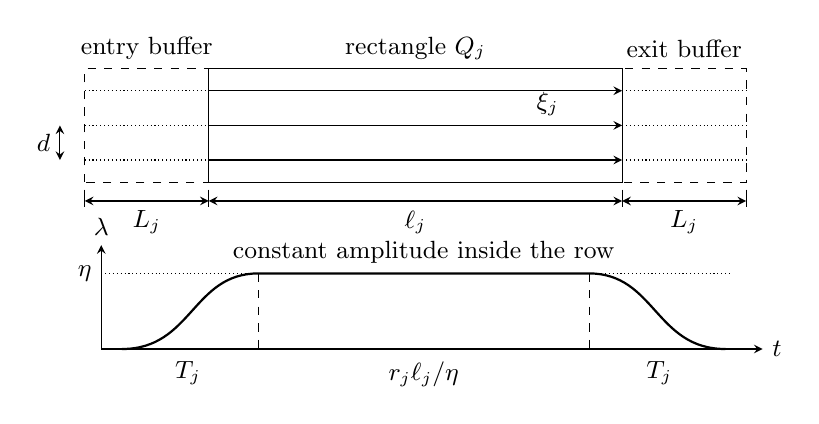
\begin{tikzpicture}[x=1.05cm,y=0.8cm,>=stealth,font=\small]
 % A rectangle and its longitudinal buffers.
 \draw[dashed] (0,0) rectangle (1.5,1.8);
 \draw (1.5,0) rectangle (6.5,1.8);
 \draw[dashed] (6.5,0) rectangle (8,1.8);
 \node at (.75,2.12) {entry buffer};
 \node at (4,2.12) {rectangle $Q_j$};
 \node at (7.25,2.12) {exit buffer};
 \foreach \y in {.35,.9,1.45} {
   \draw[densely dotted] (0,\y)--(1.5,\y);
   \draw[->] (1.5,\y)--(6.5,\y);
   \draw[densely dotted] (6.5,\y)--(8,\y);
 }
 \draw[<->] (-.3,.35)--node[left] {$d$}(-.3,.9);
 \node[above] at (5.6,.9) {$\xi_j$};
 \foreach \x in {0,1.5,6.5,8} \draw (\x,-.12)--(\x,-.4);
 \draw[<->] (0,-.3)--node[below] {$L_j$}(1.5,-.3);
 \draw[<->] (1.5,-.3)--node[below] {$\ell_j$}(6.5,-.3);
 \draw[<->] (6.5,-.3)--node[below] {$L_j$}(8,-.3);
 % Amplitude during one pass. The horizontal scales are schematic.
 \draw[->] (.2,-2.65)--(8.2,-2.65) node[right] {$t$};
 \draw[->] (.2,-2.65)--(.2,-1.0) node[above] {$\lambda$};
 \draw[densely dotted] (.2,-1.45)--(7.8,-1.45);
 \node[left] at (.2,-1.45) {$\eta$};
 \draw[thick] (.45,-2.65) .. controls (1.3,-2.65) and (1.3,-1.45) .. (2.1,-1.45)
   --(6.1,-1.45) .. controls (6.9,-1.45) and (6.9,-2.65) .. (7.75,-2.65);
 \draw[dashed] (2.1,-1.45)--(2.1,-2.65);
 \draw[dashed] (6.1,-1.45)--(6.1,-2.65);
 \node[below] at (1.25,-2.7) {$T_j$};
 \node[below] at (4.1,-2.7) {$r_j\ell_j/\eta$};
 \node[below] at (6.95,-2.7) {$T_j$};
 \node[above] at (4.1,-1.45) {constant amplitude inside the row};
\end{tikzpicture}
\caption{One dipole pass. The amplitude rises from zero in the entry
buffer, remains constant along the row, and returns to zero in the
exit buffer. The next pass can then reset the centre, direction, and
radius. A complete cycle concatenates every row pass; the diagram is
not to scale.}
\label{fig:row-pass}
\end{figure}

Fix a nonempty family in Lemma~\ref{lem:blocks}. Write each rectangle
as
\[
 Q_j=\{x_j+s\xi_j+y\xi_j^\perp:0<s<\ell_j,\ 0<y<h_j\}.
\]
Choose a smooth increasing ramp $\vartheta:[0,1]\to[0,1]$, flat at
both endpoints, with $\vartheta(0)=0$, $\vartheta(1)=1$, and
$\vartheta(s)+\vartheta(1-s)=1$. Thus
$\int_0^1\vartheta(s)\,ds=1/2$.
For each block choose an entry and exit buffer length $L_j>0$.
These lengths are fixed before the fine scale and can be chosen so that
\begin{equation}\label{eq:buffer-mass}
 M_{\mathrm{buf}}:=4\sum_j c_jh_jL_j<\sigma.
\end{equation}
The buffers extend each row longitudinally outside its rectangle;
they may intersect other rectangles, since only one dipole is active.

Let $H>0$ be small. Set
\begin{equation}\label{eq:repair-scales}
 d=H^2,\qquad\tau=H^2,\qquad
 N_j=\lfloor h_j/d\rfloor,\qquad
 y_{jk}=(k+\tfrac12)d\quad(0\le k<N_j).
\end{equation}
Take $H$ small enough that every $N_j\ge1$.
For each row use a constant radius $r_j$ and a \emph{common} peak
amplitude $\eta$ across all blocks. Define them by
\begin{equation}\label{eq:exact-schedule}
 \eta^2=\frac d{2\pi}\sum_jc_jN_j
                (\ell_j+4L_j),
 \qquad
 r_j=\frac{\tau d c_j}{2\pi\eta}.
\end{equation}
On entry, use $\lambda(t)=\eta\vartheta(t/T_j)$ for a duration
\[
 T_j=\frac{2r_jL_j}{\eta}.
\]
Because $X'=\lambda\xi_j/r_j$, the entry displacement is exactly
$L_j$. Next traverse the rectangle at amplitude $\eta$, for duration
$r_j\ell_j/\eta$, then use the reversed ramp for the exit buffer.
The amplitude is zero at the two ends of every row pass. Reset the
centre, direction, and radius there, then continue through every row
of every block.
The total time is exactly
\begin{equation}\label{eq:duration-check}
 \sum_jN_j\frac{r_j}{\eta}
             (\ell_j+4L_j)=\tau.
\end{equation}
Thus all blocks, not individual directions, form one complete cycle.

Let $M=\sum_jc_j|Q_j|$. Since $dN_j\le h_j$,
\begin{equation}\label{eq:amplitude-bound}
 \eta^2\le\frac{M+M_{\mathrm{buf}}}{2\pi}.
\end{equation}
As $H\downarrow0$, $dN_j\to h_j$, so $\eta$ tends to a positive
finite limit. Once the rectangles and buffers are fixed, there are
constants $c_0,C_0,H_0>0$ such that
\begin{equation}\label{eq:radius-scale}
 c_0H^4\le r_j\le C_0H^4<H
 \qquad\text{for every }j\text{ and }0<H<H_0.
\end{equation}
In the interior of a row $\lambda'=0$, whereas on a ramp
\[
 |r_j\lambda'|\le
  \frac{\eta^2\|\vartheta'\|_\infty}{2L_j}.
\]
Consequently
\[
 B_*:=\sup_{\mathrm{cycle}}|r\lambda'|
\]
is bounded independently of $H$ once the rectangle data and buffers
are fixed. The constants may depend on the positive coefficients
$c_j$ of this finite family; no uniform lower bound across different
families is required.

\subsection{The cycle average approximates the required stress}

On each pass use $F$ and $E$ from
\eqref{eq:visit-equation}. Since $\lambda$ vanishes at the endpoints,
\[
 \frac d{dt}\bigl(r\lambda \kappa_H(x-X(t))\bigr)
 =r\lambda'\kappa_H(x-X(t))
                    -\lambda^2\partial_\xi \kappa_H(x-X(t))
\]
implies
\begin{equation}\label{eq:cycle-average}
 \overline F:=\frac1\tau\int_{\mathrm{cycle}}F\,dt
       =\Div A_{\mathrm{av}},\qquad
 A_{\mathrm{av}}=\frac{2\pi}{\tau}\int_{\mathrm{cycle}}
        \lambda(t)^2\kappa_H(\,\cdot-X(t))\xi(t)\otimes\xi(t)\,dt.
\end{equation}
For an interior row, $dt=(r_j/\eta)\,ds$ and
$2\pi\eta r_j/\tau=dc_j$. Its contribution to
$A_{\mathrm{av}}$ is therefore the desired weighted row integral.

For completeness, for one rectangle $Q$ with side lengths $\ell,h$,
coefficient $c$, and direction $\xi$, put
\[
 F_H=cd\sum_{k=0}^{N-1}\int_0^\ell
 \kappa_H(\,\cdot-x_0-s\xi-(k+\tfrac12)d\xi^\perp)\,ds,
 \qquad N=\lfloor h/d\rfloor.
\]
Then
\begin{equation}\label{eq:rectangle-quadrature}
 \norm{F_H-c\ind_Q}1
 \le Cc\left(\frac dH|Q|+d\ell+H\operatorname{Per}(Q)\right).
\end{equation}
Here $\operatorname{Per}(Q)$ is the perimeter of $Q$. Replacing
each row by the uniform strip of width $d$ around it
costs at most $CcdH^{-1}|Q|$, using
$\|\kappa_H(\cdot-z)-\kappa_H\|_1\le C|z|/H$. The unused transverse strip
has area at most $d\ell$. Finally
\[
 \norm{\ind_Q*\kappa_H-\ind_Q}1
 \le CH\operatorname{Per}(Q),
\]
which follows directly from the area of the symmetric difference of a
rectangle and its translate. These three comparisons prove
\eqref{eq:rectangle-quadrature}.

On a ramp, $\lambda^2\le\eta^2$. Thus the combined $L^1$ norm of
all ramp contributions to $A_{\mathrm{av}}$ is at most
\[
 4\sum_j dc_jN_jL_j
 \le M_{\mathrm{buf}}.
\]
Summing \eqref{eq:rectangle-quadrature} and using $d=H^2$ gives
\begin{equation}\label{eq:average-approximation}
 \norm{A_{\mathrm{av}}-A}1
 \le M_{\mathrm{buf}}+C_{\mathrm{blocks}}H
 \qquad(0<H\le1).
\end{equation}
In particular the same small buffer mass controls both the average
error and the leading amplitude in \eqref{eq:amplitude-bound}.

\subsection{The time correction and the remaining stress}

The time correction is the time integral of the force minus its
cycle average, followed by the Leray projection
\cite[(4.76)--(4.78)]{BCK}. It vanishes at both ends of the cycle
\cite[Remark~4.1]{BCK}. If $t_*$ is the beginning of a complete
cycle, define
\begin{equation}\label{eq:time-corrector}
 z(t)=-\PP\int_{t_*}^t
                 (F(s)-\overline F)\,ds.
\end{equation}
Then $\Div z=0$, $z(t_*)=z(t_*+\tau)=0$, and
\begin{equation}\label{eq:corrector-equation}
 \partial_tz+F+\nabla p_z
                    =\overline F=\Div A_{\mathrm{av}},
\end{equation}
where
$p_z=-\Delta^{-1}\Div(F-\overline F)$ is one possible pressure.
The average in this formula is over the \emph{entire} block schedule.
A separate average over each row would not yield the tensor required
for the repair.

The $L^p$ bounds for $\PP$ and scaling of $\kappa_H$ show, for $p>1$,
\[
 \norm zp\le C_p\tau B_*H^{2/p-2}.
\]
For its curl, the identity $\curl\PP F=\curl F$ removes the
projection, so the estimate uses only
$\|\nabla \kappa_H\|_1\le CH^{-1}$.
In the norms needed below,
\begin{equation}\label{eq:corrector-bounds}
 \norm z2+\norm{\curl z}1\le C\tau B_*H^{-1}=CB_*H,
 \qquad
 \norm z{3/2}\le CB_*H^{4/3}.
\end{equation}

Let $v$ be the dipole perturbation and set $w=v+z$, the total
correction. Adding the old
Euler--Reynolds equation, \eqref{eq:visit-equation}, and
\eqref{eq:corrector-equation} gives the exact symmetric stress
\begin{equation}\label{eq:repaired-stress}
 \begin{aligned}
 \widetilde R={}&R+A_{\mathrm{av}}-qI_2+E\\
 &+u\otimes w+w\otimes u+v\otimes z+z\otimes v+z\otimes z.
 \end{aligned}
\end{equation}
The corresponding pressure is $p+p_v+p_z-q$, where $p$ is the
old pressure. Expanding $(u+w)\otimes(u+w)$ separates the old
product, the dipole product $v\otimes v$, and the five cross and
correction products displayed above.
Consequently, for a frozen tensor $S$,
\begin{equation}\label{eq:stress-estimate}
 \begin{aligned}
 \norm{\widetilde R}1\le{}&
 \norm{R-S}1+\norm{S+A-qI_2}1+
 \norm{A_{\mathrm{av}}-A}1+\norm E1\\
 &+2\norm u3\norm w{3/2}
        +2\norm v2\norm z2+\norm z2^2.
 \end{aligned}
\end{equation}
The first three errors come from approximating the stress in time
and space. The term $E$ comes from changing the dipole amplitude,
and the remaining terms are products involving the corrections.
At fixed coarse data, \eqref{eq:dipole-scaling},
\eqref{eq:visit-error}, \eqref{eq:radius-scale}, and
\eqref{eq:corrector-bounds} give
\begin{equation}\label{eq:fine-errors}
 \begin{gathered}
 \norm E1+\norm z\X\le C_{\mathrm{coarse}}H,\\
 \norm v{3/2}+\norm z{3/2}\le C_{\mathrm{coarse}}H^{4/3},\\
 \norm v\X\le C_D\eta.
 \end{gathered}
\end{equation}
Here $C_{\mathrm{coarse}}$ may depend on the fixed rectangles,
coefficients, and buffer lengths, but not on $H$. The last estimate has the universal constant
$C_D$. Once these coarse data are fixed, every fine-scale stress error
in \eqref{eq:stress-estimate} tends to zero.

\subsection{Proof of the repair lemma}

\begin{proof}[Proof of Lemma~\ref{lem:repair}]
Let $\delta=\|R\|_{L^\infty(I;L^1)}$. If $\delta=0$, take
$w=0$ and $\widetilde R=0$. Assume $\delta>0$ and fix
\[
 0<\sigma<\min\{\delta,\varepsilon/6\}.
\]
By the time-approximation assumption, choose finitely many time
cells $I_k$
and frozen symmetric tensors $S_k\in L^1$ with
\[
 \mathop{\rm ess\,sup}_{t\in I_k}\norm{R(t)-S_k}1<\sigma,
 \qquad\norm{S_k}1\le\delta+\sigma.
\]
Apply Lemma~\ref{lem:blocks} on each cell with error $\sigma$ and
choose buffers satisfying \eqref{eq:buffer-mass}. All block families
and all positive buffer lengths are now fixed. Their total core mass
is at most $C(\delta+\sigma)$ on each cell.

If a block family is empty, take $w=0$ there and
$\widetilde R=R-q_kI_2$; its norm is below $2\sigma$.
For every nonempty family, divide the time cell into $N$ equal complete
cycles and choose
\[
 \tau=|I_k|/N,\qquad H=\sqrt\tau,\qquad d=\tau.
\]
The exact schedule \eqref{eq:exact-schedule} fills each cycle.
Let $N\to\infty$, separately on each of the finitely many cells.
The first three terms in \eqref{eq:stress-estimate} have sum less
than $3\sigma+C_{\mathrm{blocks}}H$: one $\sigma$ comes from
freezing time, one from the rectangle approximation, and one from
the buffer contributions. The remaining errors tend
to zero by \eqref{eq:fine-errors} and the finite old norm
$\|u\|_{C(I;L^3)}$. Thus sufficiently large cycle counts give
$\|\widetilde R\|_{L^\infty(I;L^1)}\le\varepsilon$.

From \eqref{eq:amplitude-bound} and $\sigma\le\delta$,
\[
 \norm v\X\le C\sqrt\delta.
\]
Increasing the same cycle counts so that $\|z\|_\X\le\sqrt\delta$
gives $\|w\|_{C(I;\X)}\le C\sqrt\delta$, and hence
\eqref{eq:repair-bounds} after adjusting the universal constant.
The bound on $\|u\|_3$ only affects how small $H$ must be, not this
constant. In particular, the construction needs no additive amplitude
allowance and no derivative estimate for $u$.

This verifies the order of choices stated above: all approximation
data and buffer lengths were fixed before increasing the cycle
counts. Constants that grow when a buffer is shortened are harmless,
because the small scale is chosen after those constants are known.

It remains to justify the endpoint matching and the stated time
spaces. Each fixed
construction has finitely many passes with positive radii. Translation
continuity of $D_{r,\xi}$ in $L^2\cap L^3\cap L^{3/2}$ and of its
curl in $L^1$, together with the zero amplitude at pass endpoints,
gives the corresponding continuity of $v$. The time correction
\eqref{eq:time-corrector} is continuous in these velocity spaces, and
\[
 \curl z(t)=-\int_{t_*}^t
          \curl(F(s)-\overline F)\,ds
\]
is continuous with values in $L^1$. Both $v$ and $z$, including
their curls, vanish at complete-cycle endpoints. Therefore $w$ has
zero traces at every cell endpoint, and in particular at $a,b$.

On each fixed cell, the compact stress $E$ is continuous in
$L^1$: its coefficient $r\lambda'$ vanishes at resets and its spatial
profile is a translated fixed $L^1$ tensor. Products between perturbations are continuous in $L^1$ by their
$L^2$ continuity. Products involving the old velocity are continuous
in $L^1$ by $C_tL^3\times C_tL^{3/2}$. The remaining change
$A_{\mathrm{av}}-q_kI_2$ is constant on each cell. Thus
$\widetilde R-R$ has finitely many continuous one-sided pieces and
admits uniform time-step approximation in $L^\infty(I;L^1)$. Since
$R$ has the same approximation property, so does $\widetilde R$.

Finally, apply the equation on each time cell and add the weak
formulations. The boundary terms from $\partial_t(u+w)$ cancel
because the velocity traces agree. A jump of the stress does not
produce a temporal Dirac mass, since the equation contains only its
spatial divergence. The same argument applies at pass and cycle
boundaries. This proves the lemma on all of $I$.
\end{proof}

\section{Global iteration and the initial trace}\label{sec:global}

The endpoint condition in Lemma~\ref{lem:repair} allows us to work
on disjoint intervals. There is no need to overlap local corrections
or to differentiate a time partition of unity. We first give the
argument for a general approximate flow, so that the same result can
later be applied to the modified approximate flows used for
nonuniqueness.

\begin{proposition}[Global repair preserving values at dyadic times]\label{prop:global}
Suppose $(u^{\mathrm s},R^{\mathrm s})$ is a positive-time
Euler--Reynolds pair satisfying the approximate-flow properties
\eqref{eq:seed-properties}, with the curl bound there replaced, if
necessary, by a bound on each finite time interval. The starting
velocity need not be given by the Biot--Savart law for this
proposition. Then there is a
correction
\begin{equation}\label{eq:global-correction}
 w\in C([0,\infty);\X),\qquad w(0)=0,
\end{equation}
such that $u=u^{\mathrm s}+w$ solves \eqref{eq:weak-euler} and
\begin{equation}\label{eq:time-anchors}
 u(2^j)=u^{\mathrm s}(2^j)\qquad(j\in\mathbb Z).
\end{equation}
The solution has all the regularity properties of
Theorem~\ref{thm:main}, satisfies the Biot--Savart law, and conserves
circulation. Its $L^1$ initial vorticity trace holds whenever the
starting approximate flow has that trace.
\end{proposition}
\begin{proof}
For $j\in\mathbb Z$, put
\[
 I_j=[2^j,2^{j+1}],\qquad
 \delta_j=2^j+\sup_{t\in I_j}\norm{R^{\mathrm s}(t)}1.
\]
These numbers are positive, tend to zero as $j\to-\infty$, and are
bounded over the intervals meeting any fixed finite time horizon.

Start with $(u^{(0)},R^{(0)})=(u^{\mathrm s},R^{\mathrm s})$.
On each $I_j$, apply Lemma~\ref{lem:repair} successively, at stage $q$
with requested stress tolerance $16^{-(q+1)}\delta_j$. It gives
\begin{equation}\label{eq:dyadic-induction}
 \begin{gathered}
 u^{(q+1)}=u^{(q)}+w_q,\qquad
 \norm{R^{(q)}}{L^\infty(I_j;L^1)}\le16^{-q}\delta_j,\\
 \sup_{t\in I_j}\norm{w_q(t)}\X\le C4^{-q}\sqrt{\delta_j},
 \qquad w_q(2^j)=w_q(2^{j+1})=0.
 \end{gathered}
\end{equation}
The induction starts because $\|R^{\mathrm s}\|_{L^\infty(I_j;L^1)}
\le \delta_j$. On each compact positive-time interval only finitely many
$I_j$ occur. Thus the separate repairs paste to global positive-time
Euler--Reynolds pairs. At every finite stage the velocity is continuous
into $L^3$ on compact positive-time intervals, so the next local repair
is legitimate. No uniform-in-stage $L^3$ bound is asserted or used.

Extend every $w_q$ by zero at $t=0$. Its continuity there follows from
$\delta_j\to0$. For $T>0$, set
\[
 \delta_T^*=\sup_{j:\,2^j\le T}\delta_j<\infty.
\]
One summation controls both the velocity in $L^2$ and its curl in
$L^1$:
\begin{equation}\label{eq:graph-summation}
 \sum_{q=0}^\infty\norm{w_q}{C([0,T];\X)}
 \le C\sqrt{\delta_T^*}\sum_{q=0}^\infty4^{-q}<\infty
\end{equation}
produces $w=\sum_qw_q$ with \eqref{eq:global-correction}.
It also preserves the velocity at every dyadic time, as in
\eqref{eq:time-anchors}.
In particular
\[
 u-u_0=(u^{\mathrm s}-u_0)+w\in C([0,\infty);L^2),
 \qquad (u-u_0)(0)=0.
\]

\paragraph{The equation and its initial term.}
On compact positive-time intervals, the stresses tend to zero in
$L^\infty_tL^1_x$ and the velocities converge uniformly in local
$L^2$. For each compact spatial set $B$,
\[
 \norm{u^{(q)}\otimes u^{(q)}-u\otimes u}{L^1(B)}
 \le\left(\norm{u^{(q)}}{L^2(B)}+\norm u{L^2(B)}\right)
                      \norm{u^{(q)}-u}{L^2(B)}.
\]
Hence the limit solves Euler on $(0,\infty)$.
A continuous local $L^2$ trace extends this equation to the initial
time. Indeed, test the positive-time equation with
$\rho_\epsilon(t)\varphi(t,x)$, where $\rho_\epsilon$ increases from
zero to one on $(\epsilon,2\epsilon)$. The term with
$\rho_\epsilon'$ tends to
$\int u_0\cdot\varphi(0)\dd$ by strong local $L^2$ continuity and
$\int\rho_\epsilon'=1$. The omitted linear and quadratic integrals
tend to zero by local $L^2$ boundedness. This proves
\eqref{eq:weak-euler}.

\paragraph{Vorticity regularity.}
For $t>0$,
\[
 \mu(t)=\curl u^{\mathrm s}(t)+\curl w(t).
\]
The approximate-flow properties and \eqref{eq:global-correction}
imply
$\mu\in C((0,\infty);L^1)$ and a measure bound on every finite
horizon. At $t=0$ the curl is $\mu_0$. The identity
\begin{equation}\label{eq:limit-Hminus}
 \mu(t)=\mu_0+\curl(u(t)-u_0),\qquad
 \norm{\mu(t)}{H^{-1}}
 \le\norm{\mu_0}{H^{-1}}+\norm{u(t)-u_0}2
\end{equation}
and \eqref{eq:curl-Hminus} give strong $H^{-1}$ continuity and its
local bounds. Distributional time continuity extends to weak-*
measure continuity by uniform approximation of $C_0$ test functions
by $C_c^\infty$ functions, using the locally uniform total variation
bound. When the approximate vorticity has an $L^1$ initial trace,
\[
 \norm{\mu(t)-\mu_0}1
 \le\norm{\curl u^{\mathrm s}(t)-\mu_0}1
                      +\norm{\curl w(t)}1\longrightarrow0.
\]

\paragraph{The Biot--Savart law and circulation.}
For each fixed $t\ge0$, apply Lemma~\ref{lem:canonical} to
\[
 z=u(t)-u_0\in L^2,\qquad\nu=\mu(t)-\mu_0\in\M.
\]
It gives $z=K*\nu$ and $\nu(\R^2)=0$, hence
\[
 u(t)=K*\mu(t),\qquad\mu(t)(\R^2)=\mu_0(\R^2).
\]
The approximate-flow bounds, \eqref{eq:graph-summation}, and
\eqref{eq:limit-Hminus} also give the locally uniform bounds stated
after Theorem~\ref{thm:main}.
\end{proof}

\begin{remark}[Why the initial stress must tend to zero]
The initial correction on $I_j$ is bounded by $C\sqrt{\delta_j}$. This
tends to zero because the starting stress tends to zero. A merely bounded
initial stress would not give the strong initial velocity or
$H^{-1}$ vorticity trace by this argument. The endpoint condition is equally important: it lets us sum the
estimates independently on the dyadic intervals, with no additional
error from gluing the perturbations in time.
\end{remark}

\begin{remark}[The singular part of the initial measure]\label{rem:singular}
If $\mu_0=f\dd+\mu_0^{\mathrm{sing}}$ is the Lebesgue decomposition,
then the positive-time vorticity has an $L^1$ density, and mutual
singularity gives
\[
 \norm{\mu(t)-\mu_0}\M
  =\norm{\mu(t)-f}1+\norm{\mu_0^{\mathrm{sing}}}\M
  \ge\norm{\mu_0^{\mathrm{sing}}}\M,\qquad t>0.
\]
Thus a nonzero singular part precludes total-variation continuity at
zero for these solutions. This does not conflict with the strong
$H^{-1}$ and weak-* measure traces proved above.
\end{remark}

\section{Nonuniqueness by preserving the velocity at \texorpdfstring{$t=1$}{t = 1}}\label{sec:nonuniqueness}

\begin{proof}[Proof of Theorem~\ref{thm:main}]
Propositions~\ref{prop:seed} and~\ref{prop:global} already give one
solution with all the stated properties. To obtain infinitely many,
choose nonzero $\phi\in C_c^\infty(\R^2)$ and set
\[
 a=\nabla^\perp\phi,\qquad z_0=\Delta a,\qquad
 B_0=\nabla a+(\nabla a)^T.
\]
Then $B_0$ is symmetric, $\Div B_0=z_0$, and $\Div z_0=0$.
Moreover $z_0\ne0$, since a compactly supported harmonic $a$ would
vanish, forcing the compactly supported $\phi$ to be constant and
hence zero.

Let $(u^{\mathrm s},R^{\mathrm s})$ be the approximate flow from
Proposition~\ref{prop:seed}. Choose
$\chi\in C_c^\infty((0,\infty))$ with $\chi(1)=1$. For each integer
$n\ge1$ define
\begin{equation}\label{eq:modified-seeds}
 \begin{gathered}
 h_n=n\chi z_0,\qquad u_n^{\mathrm s}=u^{\mathrm s}+h_n,\\
 \begin{aligned}
 R_n^{\mathrm s}={}&R^{\mathrm s}+n\chi'B_0
                    +u^{\mathrm s}\otimes h_n\\
                  &+h_n\otimes u^{\mathrm s}+h_n\otimes h_n.
 \end{aligned}
 \end{gathered}
\end{equation}
Because $\partial_th_n=\Div(n\chi'B_0)$, these are exact
Euler--Reynolds pairs. The mixed stress is continuous into $L^1$ by
$C_tL^3\times C_tL^{3/2}$, and all added fields are supported away
from the initial time. The modified pairs therefore retain the
hypotheses of Proposition~\ref{prop:global}, with bounds allowed to
depend on $n$.

Repair each modified approximate flow. Since $1$ is a dyadic
endpoint, the repair leaves its velocity there unchanged:
\[
 u_n(1)=u_n^{\mathrm s}(1)=u^{\mathrm s}(1)+nz_0.
\]
For $n\ne m$,
\begin{equation}\label{eq:exact-separation}
 \norm{u_n(1)-u_m(1)}2=|n-m|\norm{z_0}2>0.
\end{equation}
The difference $u_n-u_m$ is continuous into global $L^2$, so its norm
remains positive on an interval about $1$. Thus these are distinct
space-time weak solutions, not just different representatives at an
isolated time. All have the same initial datum and every property of
the theorem.
\end{proof}


\appendix
\section{Auxiliary constructions}\label{app:auxiliary}

\subsection{A sequence for the joining times}\label{app:joining-times}

The joining argument in Section~\ref{sec:seed} needs a positive
sequence that tends to zero, controls two adjacent approximation
errors, and decreases by at most a factor of two at each step.
Here is an explicit construction, valid for every nonnegative
sequence $e_n\to0$.

Set
\[
 \gamma_k=\max\{2^{-k},\sqrt{e_k},\sqrt{e_{k+1}}\},\qquad
 \alpha_n=\sup_{k\ge0}2^{-(n-k)_+}\gamma_k,
 \qquad (s)_+=\max\{s,0\}.
\]
Then $\alpha_n\ge\gamma_n>0$, so
$\alpha_n^2\ge\max\{e_n,e_{n+1}\}$. Each term in the supremum
decreases by a factor between $1/2$ and $1$ as $n$ increases by one.
Hence
\[
 \tfrac12\alpha_n\le\alpha_{n+1}\le\alpha_n.
\]
Finally, $\gamma_k\to0$. Given $\varepsilon>0$, choose $N\ge1$ so that
$\gamma_k<\varepsilon$ for $k\ge N$. For $n\ge N$,
\[
 \alpha_n\le\max\left\{
    \max_{0\le k<N}2^{-(n-k)}\gamma_k,\ \varepsilon\right\}.
\]
The finite maximum tends to zero, proving $\alpha_n\to0$.

\subsection{The dipole profile}\label{app:dipole}

Let $J_0$ and $J_1$ be the Bessel functions of the first kind, and let
$\beta$ be the first positive zero of $J_1$. Existence of this zero
and the recurrence identities used below are classical; see
Watson \cite{Watson}. The zero is simple:
otherwise uniqueness for the Bessel differential equation at
$\beta>0$ would imply $J_1\equiv0$. The recurrence
$J_1'=J_0-J_1/z$ then gives $J_0(\beta)\ne0$.
For $x=(\rho\cos\theta,\rho\sin\theta)$, define
\begin{equation}\label{eq:dipole-stream}
 \psi(\rho,\theta)=
 \begin{cases}
 -\rho\sin\theta+
 \dfrac{2J_1(\beta\rho)}{\beta J_0(\beta)}\sin\theta,
                                      &\rho\le1,\\[4pt]
 -\dfrac{\sin\theta}{\rho},             &\rho\ge1,
 \end{cases}
 \qquad D=\nabla^\perp\psi.
\end{equation}
This is the Lamb--Chaplygin profile, with the signs fixed by our
conventions; compare~\cite[\S2.2]{BCK}. We record the verification needed
here rather than an exact energy normalization.

The Bessel identities give, from either side of $\rho=1$,
\[
 \psi=-\sin\theta,\qquad
 \partial_\rho\psi=\sin\theta,\qquad
 \partial_{\rho\rho}\psi=-2\sin\theta.
\]
Thus $D$ is $C^1$ across the boundary and smooth on either side. Set
$q=\psi+x_2$. Then
\[
 D-e_1=\nabla^\perp q,\qquad
 q|_{\partial B_1}=0,\qquad
 \curl D=-\beta^2q\ind_{B_1}.
\]
Writing $w=D-e_1$ and using
$(w\cdot\nabla)w=(\curl w)w^\perp+\nabla(|w|^2/2)$, we obtain
\[
 -\partial_1D+\Div(D\otimes D)
 =\nabla\left(\frac{|D-e_1|^2}{2}
              +\frac{\beta^2q^2}{2}\ind_{B_1}\right).
\]
The vanishing trace of $q$ excludes a boundary measure. Hence this
is an exact translating Euler profile. Outside its core,
\[
 D(x)=\nabla\left(-\frac{x_1}{|x|^2}\right),
 \qquad D(x)=O(|x|^{-2}).
\]

Rotation and scaling of the translating equation give
\eqref{eq:dipole-equation}. The bounded core, exterior decay,
and compactly supported curl give the norm scalings in
\eqref{eq:dipole-scaling}.

Define the compact radial scalar profile
\begin{equation}\label{eq:radial-density}
 W(x)=\frac1\pi\left(1-\frac{J_0(\beta|x|)}{J_0(\beta)}\right)
                          \ind_{B_1}(x).
\end{equation}
Its value and first radial derivative vanish at $|x|=1$.
Since $\int_0^1\rho J_0(\beta\rho)\,d\rho=J_1(\beta)/\beta=0$,
\[
 \int_{\R^2}W\dd=1.
\]
We now verify the radial identity \eqref{eq:dipole-projection}.
For $r=1$ and $\xi=e_1$, both sides are divergence-free $L^2$ fields,
and
\[
 \curl(2\pi\PP(We_1))=-2\pi\partial_2W
       =-\frac{2\beta J_1(\beta\rho)}{J_0(\beta)}\sin\theta
                         \ind_{B_1}=\curl D.
\]
Their difference is a divergence-free, curl-free $L^2$ field and hence
vanishes. Scaling and rotation prove \eqref{eq:dipole-projection}.


\begin{thebibliography}{99}

\bibitem{Birkhoff}
G.~Birkhoff,
\emph{Helmholtz and Taylor instability},
in \emph{Hydrodynamic Instability}, Proc. Sympos. Appl. Math.\ \textbf{13},
American Mathematical Society, Providence, RI, 1962, pp.~55--76.

\bibitem{BrueColombo}
E.~Bru\`e and M.~Colombo,
\emph{Nonuniqueness of solutions to the Euler equations with vorticity in a Lorentz space},
Comm. Math. Phys.\ \textbf{403} (2023), no.~2, 1171--1192.
DOI: \doi{10.1007/s00220-023-04816-4}.

\bibitem{BCK}
E.~Bru\`e, M.~Colombo, and A.~Kumar,
\emph{Flexibility of two-dimensional Euler flows with integrable vorticity},
Duke Math. J.\ \textbf{175} (2026), no.~9, 1593--1647.
DOI: \doi{10.1215/00127094-2025-0056}.
The section, theorem, remark, and equation numbers cited here refer to
\href{https://arxiv.org/abs/2408.07934v1}{arXiv:2408.07934v1}, 15 August 2024.

\bibitem{BuckModena}
M.~Buck and S.~Modena,
\emph{Non-uniqueness and energy dissipation for 2D Euler equations with vorticity in Hardy spaces},
J. Math. Fluid Mech.\ \textbf{26} (2024), article~26.
DOI: \doi{10.1007/s00021-024-00860-9}.

\bibitem{BuckmasterVicol}
T.~Buckmaster and V.~Vicol,
\emph{Nonuniqueness of weak solutions to the Navier--Stokes equation},
Ann. of Math.\ (2) \textbf{189} (2019), no.~1, 101--144.
DOI: \doi{10.4007/annals.2019.189.1.3}.
The pinpoint citation uses \href{https://arxiv.org/abs/1709.10033v4}{arXiv:1709.10033v4},
11 October 2018; the first preprint appeared in 2017.

\bibitem{CaflischOrellana}
R.~E.~Caflisch and O.~F.~Orellana,
\emph{Singular solutions and ill-posedness for the evolution of vortex sheets},
SIAM J. Math. Anal.\ \textbf{20} (1989), no.~2, 293--307.
DOI: \doi{10.1137/0520020}.

\bibitem{CalderonZygmund}
A.~P.~Calder\'on and A.~Zygmund,
\emph{On the existence of certain singular integrals},
Acta Math.\ \textbf{88} (1952), 85--139.
DOI: \doi{10.1007/BF02392130}.

\bibitem{Chaplygin}
S.~A.~Chaplygin,
\emph{One case of vortex motion in fluid},
Trudy Otd. Fiz. Nauk Imper. Mosk. Obshch. Lyub. Estest.\
\textbf{11} (1903), no.~2, 11--14 (Russian).
English translation, Regul. Chaotic Dyn.\ \textbf{12} (2007), no.~2, 219--232.
DOI: \doi{10.1134/S1560354707020074}.

\bibitem{CS}
G.~Crippa and G.~Stefani,
\emph{An elementary proof of existence and uniqueness for the Euler flow in localized Yudovich spaces},
Calc. Var. Partial Differential Equations \textbf{63} (2024), article~168.
DOI: \doi{10.1007/s00526-024-02750-4}.

\bibitem{DLS09}
C.~De Lellis and L.~Sz\'ekelyhidi Jr.,
\emph{The Euler equations as a differential inclusion},
Ann. of Math.\ (2) \textbf{170} (2009), no.~3, 1417--1436.
DOI: \doi{10.4007/annals.2009.170.1417}.

\bibitem{DLS10}
C.~De Lellis and L.~Sz\'ekelyhidi Jr.,
\emph{On admissibility criteria for weak solutions of the Euler equations},
Arch. Ration. Mech. Anal.\ \textbf{195} (2010), no.~1, 225--260.

\bibitem{Delort}
J.-M.~Delort,
\emph{Existence de nappes de tourbillon en dimension deux},
J. Amer. Math. Soc.\ \textbf{4} (1991), no.~3, 553--586.
DOI: \doi{10.1090/S0894-0347-1991-1102579-6}.

\bibitem{DelortSem}
J.-M.~Delort,
\emph{Existence de nappes de tourbillon pour l'\'equation d'Euler sur le plan},
S\'eminaire \mbox{\'Equations} aux d\'eriv\'ees partielles,
\'Ecole Polytechnique, 1990--1991, expos\'e~II, 12~pp.
\href{https://www.numdam.org/item/SEDP_1990-1991____A2_0/}{Numdam: SEDP\_1990-1991\_\_\_\_A2\_0}.
Page references use the printed numbering II--1, II--2, and so on.

\bibitem{DiPernaMajda87}
R.~J.~DiPerna and A.~J.~Majda,
\emph{Concentrations in regularizations for 2-D incompressible flow},
Comm. Pure Appl. Math.\ \textbf{40} (1987), no.~3, 301--345.
DOI: \doi{10.1002/cpa.3160400304}.

\bibitem{DiPernaMajda88}
R.~J.~DiPerna and A.~J.~Majda,
\emph{Reduced Hausdorff dimension and concentration-cancellation for two-dimensional incompressible flow},
J. Amer. Math. Soc.\ \textbf{1} (1988), no.~1, 59--95.
DOI: \doi{10.1090/S0894-0347-1988-0924702-6}.

\bibitem{Sparseness}
\'O.~Dom\'inguez and M.~Milman,
\emph{A sharp stability criterion for Euler equations via sparseness},
Anal. PDE \textbf{19} (2026), no.~4, 659--720.
DOI: \doi{10.2140/apde.2026.19.659}.
First preprint: \href{https://arxiv.org/abs/2310.19659}{arXiv:2310.19659} (2023).

\bibitem{DuchonRobert}
J.~Duchon and R.~Robert,
\emph{Global vortex sheet solutions of Euler equations in the plane},
J. Differential Equations \textbf{73} (1988), no.~2, 215--224.
DOI: \doi{10.1016/0022-0396(88)90105-2}.

\bibitem{Euler}
L.~Euler,
\emph{Principes g\'en\'eraux du mouvement des fluides},
M\'em. Acad. Sci. Berlin \textbf{11} (volume for 1755, published 1757), 274--315.
Enestr\"om index E226.

\bibitem{EvansMuller}
L.~C.~Evans and S.~M\"uller,
\emph{Hardy spaces and the two-dimensional Euler equations with nonnegative vorticity},
J. Amer. Math. Soc.\ \textbf{7} (1994), no.~1, 199--219.
DOI: \doi{10.1090/S0894-0347-1994-1220787-3}.

\bibitem{Holder}
E.~H\"older,
\emph{\"Uber die unbeschr\"ankte Fortsetzbarkeit einer stetigen ebenen Bewegung in einer unbegrenzten inkompressiblen Fl\"ussigkeit},
Math. Z.\ \textbf{37} (1933), 727--738.
DOI: \doi{10.1007/BF01474611}.

\bibitem{Kato}
T.~Kato,
\emph{On classical solutions of the two-dimensional non-stationary Euler equation},
Arch. Ration. Mech. Anal.\ \textbf{25} (1967), no.~3, 188--200.

\bibitem{Lamb}
H.~Lamb,
\emph{Hydrodynamics}, 3rd ed., Cambridge University Press, Cambridge, 1906.

\bibitem{NoConcentration}
M.~C.~Lopes Filho, H.~J.~Nussenzveig Lopes, and E.~Tadmor,
\emph{Approximate solutions of the incompressible Euler equations with no concentrations},
Ann. Inst. H. Poincar\'e Anal. Non Lin\'eaire \textbf{17} (2000), no.~3, 371--412.

\bibitem{Reflection}
M.~C.~Lopes Filho, H.~J.~Nussenzveig Lopes, and Z.~Xin,
\emph{Existence of vortex sheets with reflection symmetry in two space dimensions},
Arch. Ration. Mech. Anal.\ \textbf{158} (2001), no.~3, 235--257.
DOI: \doi{10.1007/s002050100145}.

\bibitem{Majda}
A.~J.~Majda,
\emph{Remarks on weak solutions for vortex sheets with a distinguished sign},
Indiana Univ. Math. J.\ \textbf{42} (1993), no.~3, 921--939.

\bibitem{Mengual}
F.~Mengual,
\emph{Non-uniqueness of admissible solutions for the 2D Euler equation with $L^p$ vortex data},
Comm. Math. Phys.\ \textbf{405} (2024), article~207.
DOI: \doi{10.1007/s00220-024-05065-9}.

\bibitem{MengualSzekelyhidi}
F.~Mengual and L.~Sz\'ekelyhidi Jr.,
\emph{Dissipative Euler flows for vortex sheet initial data without distinguished sign},
Comm. Pure Appl. Math.\ \textbf{76} (2023), no.~1, 163--221.
DOI: \doi{10.1002/cpa.22038}.
First preprint: \href{https://arxiv.org/abs/2005.08333}{arXiv:2005.08333} (2020).

\bibitem{Rott}
N.~Rott,
\emph{Diffraction of a weak shock with vortex generation},
J. Fluid Mech.\ \textbf{1} (1956), no.~1, 111--128.
DOI: \doi{10.1017/S0022112056000081}.

\bibitem{Scheffer}
V.~Scheffer,
\emph{An inviscid flow with compact support in space-time},
J. Geom. Anal.\ \textbf{3} (1993), no.~4, 343--401.

\bibitem{Schochet}
S.~Schochet,
\emph{The weak vorticity formulation of the 2-D Euler equations and concentration-cancellation},
Comm. Partial Differential Equations \textbf{20} (1995), nos.~5--6, 1077--1104.
DOI: \doi{10.1080/03605309508821124}.

\bibitem{Shnirelman}
A.~Shnirelman,
\emph{On the nonuniqueness of weak solution of the Euler equation},
Comm. Pure Appl. Math.\ \textbf{50} (1997), no.~12, 1261--1286.

\bibitem{Stein}
E.~M.~Stein,
\emph{Singular Integrals and Differentiability Properties of Functions},
Princeton Mathematical Series~30, Princeton University Press, Princeton, NJ, 1970.

\bibitem{SulemEtAl}
C.~Sulem, P.-L.~Sulem, C.~Bardos, and U.~Frisch,
\emph{Finite time analyticity for the two and three dimensional Kelvin--Helmholtz instability},
Comm. Math. Phys.\ \textbf{80} (1981), no.~4, 485--516.
DOI: \doi{10.1007/BF01941659}.

\bibitem{SzekelyhidiSheet}
L.~Sz\'ekelyhidi Jr.,
\emph{Weak solutions to the incompressible Euler equations with vortex sheet initial data},
C. R. Math. Acad. Sci. Paris \textbf{349} (2011), nos.~19--20, 1063--1066.
DOI: \doi{10.1016/j.crma.2011.09.009}.

\bibitem{VecchiWu}
I.~Vecchi and S.~J.~Wu,
\emph{On $L^1$-vorticity for 2-D incompressible flow},
Manuscripta Math.\ \textbf{78} (1993), no.~4, 403--412.
DOI: \doi{10.1007/BF02599322}.

\bibitem{VishikI}
M.~Vishik,
\emph{Instability and non-uniqueness in the Cauchy problem for the Euler equations of an ideal incompressible fluid. Part~I},
preprint, 2018, \href{https://arxiv.org/abs/1805.09426}{arXiv:1805.09426}.

\bibitem{VishikII}
M.~Vishik,
\emph{Instability and non-uniqueness in the Cauchy problem for the Euler equations of an ideal incompressible fluid. Part~II},
preprint, 2018, \href{https://arxiv.org/abs/1805.09440}{arXiv:1805.09440}.

\bibitem{Watson}
G.~N.~Watson,
\emph{A Treatise on the Theory of Bessel Functions},
Cambridge University Press, Cambridge, 1922.

\bibitem{Wiedemann}
E.~Wiedemann,
\emph{Existence of weak solutions for the incompressible Euler equations},
Ann. Inst. H. Poincar\'e Anal. Non Lin\'eaire \textbf{28} (2011), no.~5, 727--730.
DOI: \doi{10.1016/j.anihpc.2011.05.002}.

\bibitem{Wolibner}
W.~Wolibner,
\emph{Un th\'eor\`eme sur l'existence du mouvement plan d'un fluide parfait, homog\`ene, incompressible, pendant un temps infiniment long},
Math. Z.\ \textbf{37} (1933), 698--726.
DOI: \doi{10.1007/BF01474610}.

\bibitem{Yudovich}
V.~I.~Yudovich,
\emph{Non-stationary flows of an ideal incompressible fluid},
Zh. Vychisl. Mat. Mat. Fiz.\ \textbf{3} (1963), no.~6, 1032--1066 (Russian);
English translation, U.S.S.R. Comput. Math. Math. Phys.\ \textbf{3} (1963), no.~6, 1407--1456.
DOI: \doi{10.1016/0041-5553(63)90247-7}.

\end{thebibliography}
\end{document}
